\chapter{Worked Examples}
\label{chap:worked-egs}

\section{How this chapter is organised}

In developing \pharmml we have found it very useful to explain the
language using examples. By taking you through some pharmacometric models
that you are familiar with we also hope to help you understand how they
correspond to the XML representation in \pharmml. Each example is designed
to illustrate different aspects of \pharmml and our aim is that by the
end of this chapter you will understand the language and what it can
do and --- perhaps equally importantly --- what it cannot do. For
clarity and to save space we will only show key excerpts from the
examples, but the complete examples are available and will be
distributed with this document.

Figure \ref{fig:simEstTasks_List} shows an comparison in the 
structure to be implemented for a typical simulation and estimation task.
Boxes underline elements where the structure of \pharmml for these two tasks differs.

\begin{figure}[htb]
 \centering	
 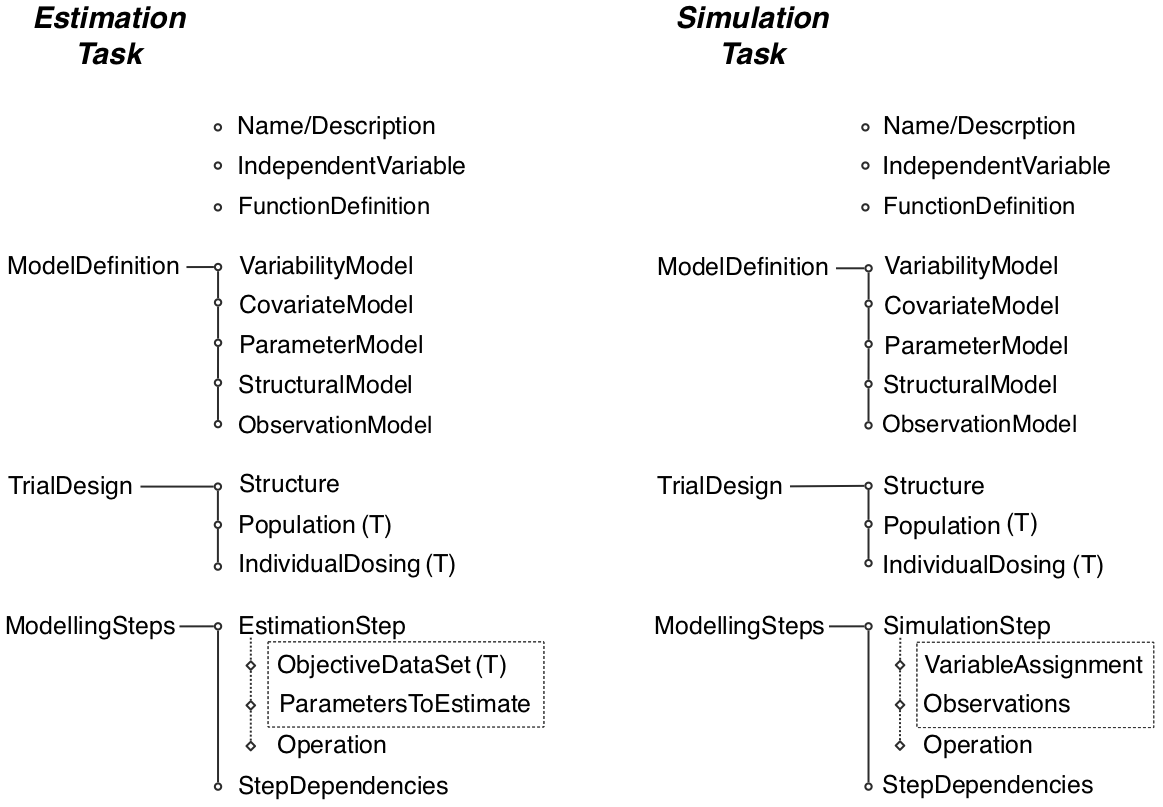
\includegraphics[width=0.8\linewidth]{pics/simEstTasks_List}%
 \caption{PharmML building blocks used in the trial definition for an estimation and simulation task. 
 Boxes underline elements where the structure of \pharmml for these two tasks differs. (T) indicates 
 that tabular data structure is used.}
 \label{fig:simEstTasks_List}
 \end{figure}

\eglabel{1}
\section{Example \theexamples: Simulation, PK + PD response}
\label{sec:eg1}

\subsection{Description}

%\subsubsection{Introduction}
\label{subsec:exp2_intro}

The following example is based on the CTS1 use case
\cite{Lavielle:2011}. Both PK (the drug concentration) and PD (the
drug effect) are simulated. A one compartment PK model is linked to an
indirect response PD model, see Figure \ref{fig:simplePKPD} for a typical 
simulation result for one patient.

\begin{figure}[ht!]
\begin{center}
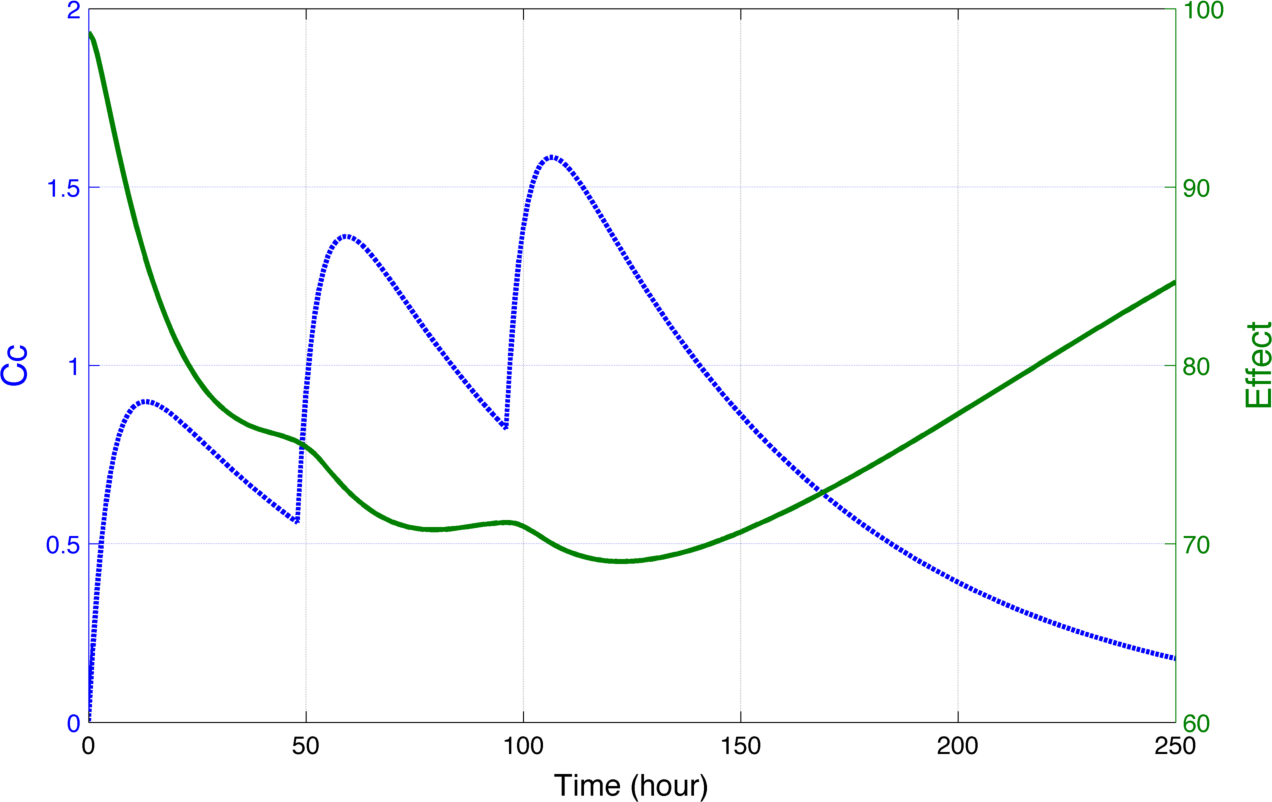
\includegraphics[width=.45\textwidth]{pics/CTS1_smallPKPD}
\caption{Simulated combined model as defined in the example with PK (blue) and PD (green) time courses for one subject. Here three doses were administered every $48h$.}
\label{fig:simplePKPD}
\vspace{-20pt}
\end{center}
\end{figure}

\subsubsection{Model Definition}

\paragraph{Structural model}
This is an oral one compartment model and an indirect response model
with parameters \var{ka}, \var{V}, \var{CL}, \var{Imax}, \var{IC50},
\var{Rin} and \var{kout}.

\begin{align}
k&=\frac{\CL}{V}  \label{eqn:eg1-struct-model}\\
\frac{dAd}{dt} &=-ka \times Ad  \nonumber\\
\frac{dAc}{dt}&=ka \times Ad - k \times Ac  \nonumber\\
\frac{dE}{dt} &=Rin \times \Bigg(1-\frac{\Imax \times \Cc}{\Cc+\IC50}\Bigg)
- kout \times E \nonumber\\
\Cc &= \frac{Ac}{V} \nonumber
\intertext{initial conditions:}
E(t=0) &= \frac{Rin}{kout}  \label{eqn:eg1-init-conds}\\
Ad(t=0) &= 0  \nonumber\\
Ac(t=0) &= 0 \nonumber
\end{align}


\paragraph{Covariate model}

The only covariate is Weight, $W$, and it is a continuous covariate:
\begin{gather}
W \sim \mathcal{N}(\pop_{\Weight}, \omega_{\Weight}) \label{eqn:eg1-covariate-defn}
\intertext{The following transformation is applied:}
\log(\Weight/70) \label{eqn:eg1-covariate-trans}
\intertext{and the initial values are:}
\pop_{\Weight} =70.07, \quad \omega_{\Weight} =14.09 \nonumber
\end{gather}

\paragraph{Parameter model}

\subparagraph{PK parameters}

The model uses the following individual parameters:
\begin{description}
\item[\var{ka}] absorption rate constant
\item[\var{V}] volume of distribution
\item[\var{CL}] clearance of elimination
\end{description}
All follow a log-normal distribution:
\begin{align}
\log(ka_{i}) &=  \log(\pop_{ka}) + \eta_{ka,i}   \label{eqn:eg1-param-ka}\\
\log(V_i) &= \log(\pop_{V}) + \beta_{1,V}\log(W_i/70) + \eta_{V,i}   \label{eqn:eg1-param-V}\\
\log(\CL_i) &=  \log(\pop_{\CL}) + \beta_{1,\CL}\log(W_i/70) +
\eta_{\CL,i} \nonumber
\end{align}
where
\begin{gather*}
\eta_{ka,i} \sim N(0, \omega_{ka}), \quad \eta_{V,i} \sim N(0,
\omega_{V}), \quad \eta_{\CL,i} \sim N(0, \omega_{\CL})
\intertext{with initial values:}
\pop_{ka}=1,\quad \omega_{ka}=0.6  \qquad \pop_V=8,\quad \omega_V=0.2 \\
\pop_{\CL}=0.13,\quad \omega_{\CL}=0.2  \qquad \beta_{1,V}=1 , \quad \beta_{1,\CL}=0.75  \\
\rho_{V,\CL}=0.7\footnotemark
\end{gather*}
\footnotetext{Correration coefficient between $\eta_{V,i}$ and $\eta_{\CL,i}$}

\subparagraph{PD parameters}

The model uses the following individual parameters:
\begin{description}
\item[\var{Imax}] maximal antagonistic response
\item[\var{IC50}] concentration giving half the maximal response
\item[\var{Rin}] input (synthesis) rate
\item[\var{kout}] output (elimination) rate
\end{description}
All follow a log-normal distribution, except \var{Imax}, which follows a logit-normal distribution.
\begin{align*}
\logit(Imax_i) =& \logit(\pop_{Imax})  + \eta_{Imax,i}   \\
\log(\IC50_{i}) =& \log(\pop_{\IC50}) + \eta_{\IC50,i}  \\
\log(\Rin_i) =& \log(\pop_{\Rin}) + \eta_{\Rin,i}  \\
\log(\kout_i) =& \log(\pop_{\kout}) + \eta_{\kout,i}
\end{align*}
where
\begin{gather*}
  \eta_{Imax,i} \sim N(0, \omega_{Imax}), \quad \eta_{\IC50,i} \sim
  N(0, \omega_{\IC50}), \\
\eta_{\Rin,i} \sim N(0, \omega_{\Rin}), \quad \eta_{\kout,i} \sim N(0, \omega_{\kout})
\intertext{with initial values:}
\pop_{Imax} =0.9,\quad \omega_{Imax}=2  \qquad \pop_{\IC50} =
0.4,\quad \omega_{\IC50} =0.4  \\
\pop_{\Rin}=5, \quad \omega_{\Rin}=0.05  \qquad \pop_{\kout} =0.05,
\quad \omega_{\kout} =0.05
\end{gather*}

\paragraph{Variance-covariance matrix}
\label{sec:covariance-matrix}
The full variance-covariance matrix for the random effects is:
\begin{gather}
 \Omega =
 \begin{pmatrix}
  \omega_{ka}^2 	& 0 				& 0  				& 0  				& 0  				& 0  				& 0  				\\
   			  	& \omega_{V}^2	& \omega_{V,\CL} 	& 0  				& 0  				& 0  				& 0  				\\
  				& 				& \omega_{\CL}^2	& 0  				& 0  				& 0  				& 0  				\\
 				&				&   				& \omega_{Imax}^2  & 0  				& 0  				& 0  				\\
				&   				&   				&   				& \omega_{IC50}^2  & 0  				& 0  				\\
				&   				&   				&   				&   				& \omega_{Rin}^2 	& 0  				\\
				&   				&   				&   				&   				&   				& \omega_{kout}^2
 \end{pmatrix}
\intertext{where}
\omega_{V,\CL} = \omega_\var{V} \, \omega_{\CL} \,\rho_{\var{V},\CL}\nonumber
\label{sec:eg-covariance-mat}
\end{gather}

\paragraph{Observation model}
\label{sec:eg1-desc-obs-model}

We apply a residual error model to the output variables \var{Cc} and \var{E}
from the PK and PD models respectively.

%\begin{table*}[h!]
\begin{center}
\begin{tabular*}{0.8\linewidth}{@{\extracolsep{\fill}} >{\bfseries}l l l}\toprule
Output Variable & \textbf{\itshape Cc} &\textbf{\itshape E}\\\midrule
Observation Name & Concentration & PCA\\
Units & $\mg/l$ & $\%$\\
Type & Continuous & Continuous \\
Model & Combined & Constant \\
Parameters & $a = 0.5,\quad b=0.1$ & $a=4$\\
\bottomrule
\end{tabular*}
\end{center}

%%%%%%%%%%%%%%%%%%%%%%%%%%%%%%%%%%%%%%%%%%%%%%%%%%%%%%%%%%%%%%%%
\subsubsection{Trial Design}
\label{subsec:exp2_TaskDescription}

\begin{figure}[h!]
\centering
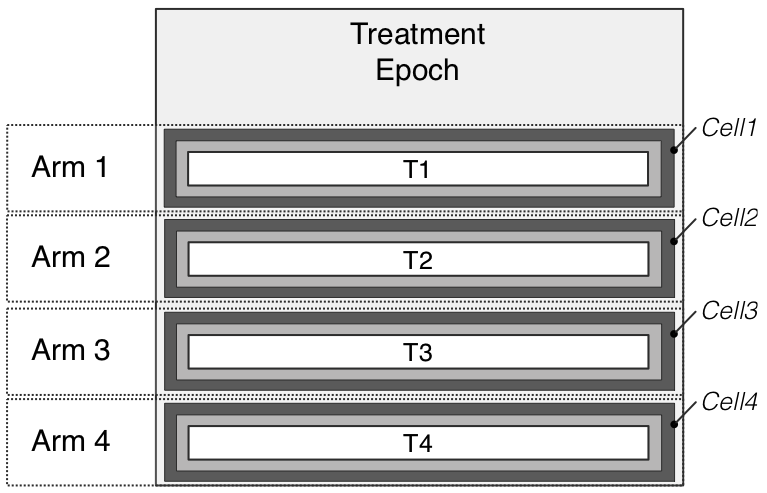
\includegraphics[width=0.7\linewidth]{../pics/designPattern_4Arms1Epoch}
\caption{Design overview: this study consists of four arms and one epoch. The differences between arms lie in the number of subjects, dose amount and times. See table below for the details.}
\label{fig:designPattern_4Arms1Epoch}
\end{figure}

Figure \ref{fig:designPattern_4Arms1Epoch} shows the \textit{Structure} of
this example consisting of four arms and one epoch, meaning there are four treatment
types for which only one time period needs to be specified.

The dosing regimen for the trial is given for each arm below. Note
that all dosing is bolus dosing (discrete administration at specific
times) and all doses are administered to the same compartment.

%\begin{table*}[h!]
\begin{center}
\begin{tabular*}{0.9\linewidth}{@{\extracolsep{\fill}} >{\bfseries}l rrrr}\toprule
Arm & \textbf{1} &\textbf{2} &\textbf{3} & \textbf{4}\\\midrule
Number of subjects & 20 & 20 & 40 & 40 \\
Dose target & \var{Ad} & \var{Ad} & \var{Ad} & \var{Ad}\\
Dosing Amount & 0.25 & 0.5 & 0.5 & 1\\
Dose Units & $\mg/\kg$  & $\mg/\kg$  & $\mg/\kg$  & $\mg/\kg$ \\
Dose per kg & yes & yes & yes & yes\\
Dosing times (h) & 0:24:192 &  0:48:192 &  0:24:192 & 0:48:192 \\
\bottomrule
\end{tabular*}
\end{center}


%%%%%%%%%%%%%%%%%%%%%%%%%%%%%%%%%%%%%%%%%%%%%%%%%%%%%%%%%%%%%%%%
\subsubsection{Modelling Steps}

Time of measurement for PK and PD happens according to different
schedules and these observation time points are produced by the
simulation. The output variables to be generated by the simulation and
their associated time points are shown below:

\begin{center}
\begin{tabular*}{0.9\linewidth}{@{\extracolsep{\fill}} >{\bfseries}l c c}\toprule
Output Variable & \textbf{\itshape Cc} &\textbf{\itshape E}\\\midrule
Observation times & [0.5,4 : 4 : 48,52 : 24 : 192,192 : 4 : 250] & 0 : 24 : 288\\
\bottomrule
\end{tabular*}
\end{center}

%%%%%%%%%%%%%%%%%%%%%%%%%%%%%%%%%%%%%%%%%%%%%%%%%%%%%%%%%%%%%%%%
\subsection{\pharmml Document Structure}
\label{sec:symbol-defn}
An overview of the model with the key sections collapsed  as shown in this listing
\inputxml{exp1_lst1.xml}
illustrates the main sections of the model as described
in section \ref{sec:structure-overview}. The key points to note are
the use of the \xatt{independentVar\-iable}  attribute to set the time
variable to $t$ (c.f.\xspace section \ref{sec:independent-var}), and
how the element \texttt{Name} defines the name of the model. In addition
the top-level \texttt{PharmML} element contains a number of attributes
prefixed \texttt{xmlns}. These are required by the XML Schema standard
and can be ignored as we go through the examples\footnote{If you
  want to learn more about the technical aspects of XML and the XML Schema standard
  used to define \pharmml then we recommend to start here:
  \url{http://www.w3.org/TR/xmlschema-0/}. And, by the way,
  \texttt{xmlns} stands for XML namespace.}.

%\begin{listing}[htb]
%\inputxml{exp1_lst1.xml}
%\caption{An overview of the \pharmml document for example \egref{1}.}
%\label{eg:eg1-overview}
%\end{listing}

The above listing introduces a concept and XML element that we did not describe
before: this is the \xelem{FunctionDefinition} element. It defines a function that
returns a real type as shown in the following listing 
%\ref{eg:symboldefn}. 
\inputxml{exp1_lst2.xml}

The function takes three arguments of scalar type and defines the
function:
\begin{displaymath}
\var{combinedError}(a, b, f) = a + bf
\end{displaymath}
This function is used to encode the combined error model function used later in
the observation model (see section \ref{sec:eg1-obs-model}).

%\begin{listing}[htb]
%\inputxml{exp1_lst2.xml}
%\caption{Function definition using the \xelem{FunctionDefinition} element.}
%\label{eg:symboldefn}
%\end{listing}

%%%%%%%%%%%%%%%%%%%%%%%%%%%%%%%%%%%%%%%%%%%%%%%%%%%%%%%%%%%%%%%%%
%\subsubsection{Units}
%\label{sec:eg1-units}
%
%Listing \ref{eg:eg1-units} shows how we define units for this example, see for details \ref{sec:units}. It is done using the element \xelem{UnitDefinition} and child element \xelem{UnitComponent}. For example $mg$ for tumour mass or $mg/kg$ as dose unit to express the dosing per kilogram of body weight.
%
%\begin{listing}[htb]
%\inputxml{exp1_units.xml}
%\caption{Examples of the units definition in example \egref{1}.}
%\label{eg:eg1-units}
%\end{listing}
%


%%%%%%%%%%%%%%%%%%%%%%%%%%%%%%%%%%%%%%%%%%%%%%%%%%%%%%%%%%%%%%%%
\subsection{Model Definition}

As you can see in the following listing 
\inputxml{exp1_lst3.xml}

the model definition section defines the main components that you will see in
the subsequent examples. Apart from the structural model, all of these
elements are optional and all follow the scoping rules described in
section \ref{sec:blocks}.

%\begin{listing}[htb]
%\inputxml{exp1_lst3.xml}
%\caption{Overview of the Model Definition section in example \egref{1}.}
%\label{eg:eg1-modeldefn-overview}
%\end{listing}

%\begin{listing}[htb]
%\inputxml{exp1_lst3A.xml}
%\caption{In example \egref{1} there are two variability models, one related
%to the IIV and one related to the residual error.}
%\label{eg:eg1-residualAndIndividual}
%\end{listing}


%%%%%%%%%%%%%%%%%%%%%%%%%%%%%%%%%%%%%%%%%%%%%%%%%%%%%%%%%%%%%%%%
\subsubsection{Variability Model}
\label{sec:eg1-variability}

\begin{figure}[ht!]
\centering
 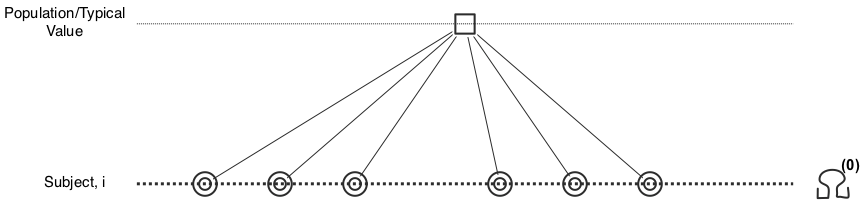
\includegraphics[width=120mm]{tree_IOV0}
\caption{There is only one level of variability in this example -- inter-individual variability.}
\label{fig:tree_IOV0}
\end{figure}

From the listing above one can also see that there
are two variability models defined using the element
\xelem{Vari\-abilityModel}. This is how we explicitly define the
level of variability in the model (c.f.\ section
\ref{sec:variabilityModel}). In this case there is one level of 
variability, the inter-individual, Figure \ref{fig:tree_IOV0} and the residual
error model variability, see the following listing \inputxml{exp1_lst3A.xml}
for the details of the implementation. Please, note that we use two different variability 
attribute types, \xatt{model} and \xatt{error}. The former stands for random variability
associated with the parameters, as described in section \ref{sec:variabilityModel}. 
For this example we are defining one level of variability in the parameter model and this
corresponds to variability between subjects. The latter stands for residual error variability.

We will explain this more fully below when we look at
examples with more complex variability models (section
\ref{eg6:variabilityModel}).

%%%%%%%%%%%%%%%%%%%%%%%%%%%%%%%%%%%%%%%%%%%%%%%%%%%%%%%%%%%%%%%%
\subsubsection{Covariate Model}
\label{sec:eg1-covariate}


The \xelem{CovariateModel} block corresponds to the covariate model
defined in section \ref{maths:covariate_model}. In this example, as shown
in this listing \inputxml{exp1_lst4and5.xml}
we are defining a continuous
covariate, \var{W}, indicated by the \xelem{Continuous} element and
the covariate is sampled from a normal distribution as in equation
\ref{eqn:eg1-covariate-defn}.  The element \xelem{Transformation}
beneath the definition of the distribution describes the
transformation applied to this covariate whenever it is used. In this
case the transformation being applied is defined in
equation~\ref{eqn:eg1-covariate-trans}.

%\begin{listing}[htb]
%\inputxml{exp1_lst4and5.xml}
%\caption{The Covariate Model}
%\label{eg:eg1-covariate-model}
%\end{listing}



%%%%%%%%%%%%%%%%%%%%%%%%%%%%%%%%%%%%%%%%%%%%%%%%%%%%%%%%%%%%%%%%
\subsubsection{Parameter Model}
\label{sec:eg1-pk}
All parameters in the current example \egref{1} can be defined
using the Gaussian model with linear covariates (see section
\ref{sec:parameterModel}). We will start with a simple case in this
example, shown in the following listing \inputxml{exp1_lst6.xml}
the absorption rate constant \var{ka}. 
First the typical value for \var{ka}, \var{pop\_ka}
and the standard deviation of the random effect, \var{\omega\_ka}, are
defined as \xelem{SimpleParameter}'s. Then the random effect \var{eta\_ka}
is defined, and it follows a normal distribution with mean $0$ and
standard deviation \var{\omega\_ka}.

Then the actual individual parameter \var{ka} is
defined with the \xelem{Transformation} attribute set to
\texttt{log}. This tells us that the parameter is log-transformed. We
are using the Gaussian model described previously (section
\ref{maths:parameter-model}), and it follows a log-normal distribution
with the mean \var{pop\_ka} and the standard deviation
 \var{omega\_ka}, as shown in equation \ref{eqn:eg1-param-ka}.
Even though \var{ka} is modelled without a covariate, we still use the
element \xelem{LinearCovariate}, which contains here logically only the
typical value element \xelem{PopulationParameter}.

%\begin{listing}[htb]
%\inputxml{exp1_lst6.xml}
%\caption{A simple parameter definition: parameter $ka$.}
%\label{eg:eg1-param-prt1}
%\end{listing}

The \xelem{RandomVariable} element is very important here. It tells us
what the random effect is, and, by assigning a variability level to
the attribute \xatt{symbIdRef} within the \xelem{VariabilityRef\-erence} element,
it effectively tells us that the random effect is sampled for every subject.
The importance of this will become clearer in later examples that describe
multiple levels of variability. Note that the \xelem{RandomVariable} element
also defines a new symbol \var{eta\_ka}, which is a parameter.


%\begin{listing}[htb]
%\inputxml{exp1_lst7.xml}
%\caption{A more complicated parameter definition: parameter $V$.}
%\label{eg:eg1-param-prt2}
%\end{listing}

Of course not all parameter definitions are so straight forward. In the
following listing \inputxml{exp1_lst7.xml}
you can see the definition of a
parameter, \var{V}, that is related to the covariate, $W$. We do this
using the element \xelem{Covariate} to indicate there is a
relationship. Then we reference the specific covariate (using the
\xelem{SymbRef} element) and describe the fixed effect relating the
covariate to this parameter: in this case we are referring to the
parameter \var{beta\_V}. We define here a linear covariate model
when relating covariates to parameters (c.f.\xspace section
\ref{maths:covariate_model}), so this example corresponds to
equation \ref{eqn:eg1-param-V}.

You may have noticed that in equation \ref{eqn:eg1-param-V} the
covariate term is $\log\left(W/70\right)$ and not \var{W}. Why? Well
we have applied the covariate transformation defined in
(\ref{eqn:eg1-covariate-trans}). As we described above (section
\ref{sec:eg1-covariate}), whenever a covariate is used here we always
apply any transformation defined in the \xelem{Transformation}
element.

Having defined the individual and other parameters in the parameter
model we need to describe the correlation of the random effects, if any.
As described above (see section \ref{subsec:correlationModel} for
a complete description) we do this using a covariance matrix.
In \pharmml, if the random effects of both
parameters follow a normal distribution, then we assume that the
diagonal of the covariance matrix can be derived from the variance or
standard deviation of each parameter (c.f section
\ref{maths:covariance-mat-derivation}). This is true in our example,
so we only need to define the parts of the covariance matrix that
define the correlation between parameters \var{V} and \var{CL}
as shown in this listing \inputxml{exp1_lst8.xml}
Notice that with the
\xatt{symbIdRef} attribute the correlation is associated with the
variability level defined at the beginning of the model
definition. This allows us to define a covariance matrix for each
level of variability in the model and thus to define different
parameter correlations at each level as well. This single
\xelem{Correlation} element is all we need to define the covariance
matrix mentioned above (section \ref{sec:eg-covariance-mat}).

%\begin{listing}[htb]
%\inputxml{exp1_lst8.xml}
%\caption{The correlation of parameters \var{V} and \var{CL}.}
%\label{eg:eg1-param-prt3}
%\end{listing}

You now know most of the structures used to define a parameter in
\pharmml. As you will see later, these elements can be combined to
create more complicated parameter models, but these are elaborations
of this framework.

%%%%%%%%%%%%%%%%%%%%%%%%%%%%%%%%%%%%%%%%%%%%%%%%%%%%%%%%%%%%%%%%
\subsubsection{Structural Model}

In \pharmml the structural model can be described using algebraic
equations or an ODE system. In this example the
model is defined as a combination of an ODE system and
some supporting algebraic equations (c.f.\xspace equation \ref{eqn:eg1-struct-model}).

%\begin{listing}[htb]
%\inputxml{exp1_lst9and10.xml}
%\caption{A subset of the structural model showing how variables
%  \var{k} and \var{Ad} are defined and how we specify the initial condition for a
%  variable defined by an ODE.}
%\label{eg:eg1-struct-prt1}
%\end{listing}

The following listing \inputxml{exp1_lst9and10.xml} illustrates how the variable \var{k}
is defined. We cover this in more detail in chapter
\ref{chap:lang-overview}, but briefly: \var{k} is defined as having a
real type and is assigned the result of the expression $CL/V$, which
are parameters defined in the parameter model, \var{p1}. We can also
see how the derivative \var{Ad} is defined using the element \xelem{DerivativeVariable}
(see section \ref{sec:odes} for a more detailed explanation)
with $t$ as the independent variable. The full ODE defined is:
\[
\frac{\mathrm{d}\,\var{Ad}}{\mathrm{d}t} = -\var{ka} \, \var{Ad}
\]
where \var{ka} is a parameter defined in the parameter model \var{p1}.
Finally the \xelem{InitialCondition} element defines
the initial value for \var{Ad} at time 0, here $Ad(t\!=\!0)\!=\!0$, which is the default initial time
in \pharmml.
%\begin{listing}[htb]
%\inputxml{eg1_struct_model_prt2.xml}
%\caption{Defining the initial conditions of the model.}
%\label{eg:eg1-struct-prt2}
%\end{listing}
%
%Since this defines a system of differential equations, we need to
%define the initial conditions. Second part of listing \ref{eg:eg1-struct-prt1} shows
%how the initial conditions in equation \ref{eqn:eg1-init-conds} are defined
%in \pharmml. Very simply the result of a mathematical expression described in
%\pharmml Maths is assigned to the variables at $t=0$.

%%%%%%%%%%%%%%%%%%%%%%%%%%%%%%%%%%%%%%%%%%%%%%%%%%%%%%%%%%%%%%%%
\subsubsection{Observation Model}
\label{sec:eg1-obs-model}

In this example there are two observations for the continuous
variables \var{Cc} and \var{E}, which are outputs from the structural
model. As described above each has a residual error model applied to it.

%\begin{listing}[htb]
%\inputxml{exp1_lst11.xml}
%\caption{The residual error model applied to variable \var{Cc}.}
%\label{eg:eg1-obs}
%\end{listing}

The XML is very similar for both variables so in the following listing 
%\ref{eg:eg1-obs} 
\inputxml{exp1_lst11.xml}
we only show how the residual error model for \var{Cc}, the continuous PK variable, is defined.
First the parameters of the residual error model \var{a} and \var{b} are
defined using \xelem{SimpleParameter}; here a combined additive
and proportional error model is applied. Then \var{epsilon\_Cc} as \xelem{RandomVariable}
of the residual error model with a mean of $0$ and standard deviation \var{sigma\_Cc} is defined
to be used in the subsequent parts of the model. Note that we need to 
indicate the type and level of the according random effect which were
defined in the 'Variability Model' section above. This is done
using the \xelem{VariabilityReference} 

The subsequent element \xelem{Standard} states that we are defining a standard
continuous observation model. This means in short that we can define
an observation model of the form $y_{ij} = f_{ij} + g\times\epsilon_{ij}$
(for details, see the discussion below and section \ref{sec:observationModel}).

The attribute \xatt{symbId} of \xelem{Standard} defines the name of the
variable that will hold the result of the applied residual error model.
The \xelem{Output} element then defines the
variable in the structural model that the residual error model applies to
(in this case \var{Cc}). Next we define the actual residual error
model with the \xelem{ErrorModel} element. The error model is invoked
by calling the function \var{combinedErrorModel} defined in the symbol
definition at the beginning of the \pharmml document (see section
\ref{sec:symbol-defn}). We pass in the appropriate parameter values
(see section \ref{maths:combined-err-model} for a description of the
residual error model) and this defines our residual error model.\\
Finally we use the \xelem{ResidualError} element to reference the
\var{epsilon\_Cc} specified before.



%%%%%%%%%%%%%%%%%%%%%%%%%%%%%%%%%%%%%%%%%%%%%%%%%%%%%%%%%%%%%%%%%%
\paragraph{Residual model implementation}
Most residual error model types have two or three equivalent forms, by which 
we mean they have the same variance, although they use one or more residual 
errors, $\epsilon_{ij}$, see examples in section \ref{subsec:modelExamples}. 
Other types contain two or more predictions from the structural model, \var{f_{ij}}. 
From a computational point of view it makes a lot of sense to reflect such 
differences in the language structure.
This was the motivation to allow for the implementation of two types of observation models
\begin{itemize}
\item
\xelem{Standard} -- any observation model of the form
\begin{align*}
	u(y_{ij}) = u(f_{ij}) + g\times\epsilon_{ij}
\end{align*}
which can be defined using exactly one of the following items
\begin{itemize}
\item
a transformation, $u$, e.g. \var{log} or \var{logit}
\item
one structural model prediction, \var{f_{ij}}
\item
one standard deviation function, \var{g}
\item
one random variable, $\epsilon_{ij}$
\end{itemize}
\item
\xelem{General} -- using any number of the items listed above and arbitrary functional relationship between them.
\end{itemize}
This chapter contains more examples illustrating these constructs.

%We described in chapter \ref{chap:mathsdefn} (section
%\ref{sec:residualErrorModel}) how we currently assume the residual
%error model to be of the form $g\epsilon$, where $g$ is the error
%model and $\epsilon$ is a random value sampled from a probability
%distribution. In \pharmml (listing \ref{eg:eg1-obs}) the
%\xelem{RandomEffect} element defines $\epsilon$. This element is
%similar to its namesake in the parameter model in that it describes a
%probability distribution, but in this case it is not associated with a
%level of variability nor do we assign it symbol name. In the listing
%the distribution was omitted to save space, but it is defined in
%exactly the same way as it is in the parameter model.

%%%%%%%%%%%%%%%%%%%%%%%%%%%%%%%%%%%%%%%%%%%%%%%%%%%%%%%%%%%%%%%%
\subsection{Trial Design}
\subsubsection{Structure}

In this fairly simple case, there is only one epoch and four arms, \var{Arm\_1}, \var{Arm\_2} etc.,
cf. Figure \ref{fig:designPattern_4Arms1Epoch}.
The resulting four cells \var{Cell\_1}, \var{Cell\_2} etc. each correspond
to one arm and contain one segment.
Figure \ref{fig:CellSegmentEpochArm_example1} (right) illustrates the inter-relationship between
cells, arms, epochs and segments. Here a segment consists of one activity --
a certain type of treatment. In general, a segment can contain more
than one activity. Dosing regimen can be defined for different
compartments in the structural model. In this example there are four
treatments with one dosing regimen per treatment.

\begin{figure}[htbp!]
\centering
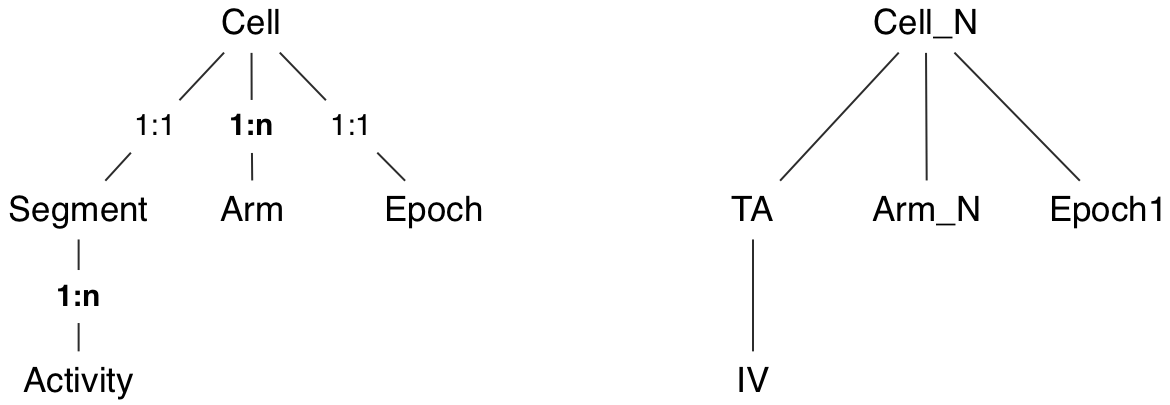
\includegraphics[width=0.7\linewidth]{pics/CellSegmentEpochArm_example1}
\caption{(left) General cell hierarchy; (right) How it is applied in example \egref{1}.
There is only one epoch and four arms, \var{Arm\_1}, \var{Arm\_2} etc.
The resulting four cells \var{Cell\_1}, \var{Cell\_2}, etc. each correspond
to one arm and contain one segment. See the listing bellow for how
these features are implemented and structured.}
\label{fig:CellSegmentEpochArm_example1}
\end{figure}

%The treatment in \pharmml is used to describe the dosing regimen
%applied to the subjects in the trial. A treatment can contain more
%than one dosing regimen and drugs can be administered to different
%compartments in the structural model. In this example there are four
%treatments with one dosing regimen per treatment.

%\begin{listing}[htb]
%\inputxml{exp1_lst12.xml}
%\caption{A treatment with bolus dosing.}
%\label{eg:eg1-treatment}
%\end{listing}

%\ref{eg:eg1-treatment} 
In the following listing 
\inputxml{exp1_lst12.xml} we show an activity defined for \var{Arm\_1},
here treatment in the form of a bolus administration: the others are very similar.
The \xelem{Activity} element is given an identifier, ``\texttt{d1}'',
and the element \xelem{Bolus} defines a
bolus administration\footnote{Bolus and infusion are the only types of
dosing regimen permitted. We make no distinction between oral and IV
administration as such differences are handled by the structural
model used.}.  \xelem{DoseAmount} defines the amount of drug to be
administered. The are basically two options here. Either the dose is assigned
to the variable defined by an ODE, such is the case here, for which we use
\xatt{inputType="target"} attribute or the dosing variable \var{D} as in algebraic
equations. 
Additionally, in this case the administration is adjusted for body
weight using the expression $0.25W$. The element \xelem{SymbIdRef}
defines the target of dosing. This effectively defines an input
function that adds the dose amount
to the variable \var{Ad} at the specified dosing time. The dosing
times themselves are given by the \xelem{DosingTimes} element as the
sequence $0:24:192$.
% (see section \ref{sec:arrays} for more information about sequences).

%%%%%%%%%%%%%%%%%%%%%%%%%%%%%%%%%%%%%%%%%%%%%%%%%%%%%%%%%%%%%%%%%
%\subsubsection{Treatment Epoch and Group}

%In this example (listing \ref{exp1_lst13}) the purpose of the
%Treatment Epoch is not clear. In general the treatment epoch provides
%a time-frame that dosing times are relative to, and this permits us to
%define more complex trial design structures as you will see in later
%examples. However, in this simple example no time-frame is defined so
%it is assumed to be the interval $[0, \inf]$ (see section
%\ref{maths:epoch-defn}). The epoch can contain one or more treatments,
%which are referenced using the \xelem{TreatmentRef} element.

%\begin{listing}[htb]
%\inputxml{exp1_lst13.xml}
%\caption{Arm, cell, epoch and segment/activity definition (see Figure
%\ref{fig:CellSegmentEpochArm_example1} for the relationship between
%these elements).}
%\label{exp1_lst13}
%\end{listing}

Once the segments with their according treatments/activities are defined, we can define epochs using the
element \xelem{Epoch} with their start and stopping time along with their order.
After the arms are specified, the \xelem{Cell} element is used to put all of the components together, see this listing 
\inputxml{exp1_lst13.xml}

%%%%%%%%%%%%%%%%%%%%%%%%%%%%%%%%%%%%%%%%%%%%%%%%%%%%%%%%%%%%%%%%
\subsubsection{Population}

The \xelem{Population} is the second and in the case of a simulation example,
also the last block in the trial design definition. As explained in chapter \ref{sec:CTS}
this is the place to define the number of subjects per study arm, constant
or time-varying covariates and other properties, if available.
In this particular case covariates are simulated according to 
the definition in eq.\ref{eqn:eg1-covariate-defn}. This is the reason the following table with 
population data will have only three columns. (In case of estimation the covariates would have to 
be listed explicitly in this table as well, this will be described in the next example \ref{sec:eg4})\\
The definition of the table is in the \xelem{IndividualTemplate} block where the columns
\var{id}, \var{arm} and \var{reps} are specified, see the following listing 
\inputxml{exp1_lst13A.xml}
Using the \var{reps} variable allows us
to shorten the definition in cases where all other features are the same across subjects in
an arm, which is the case here. Here four arms with 20, 20, 40 and 40 subjects, respectively, are defined.
An alternative would be to list all subjects explicitly, in which case only two columns would be
sufficient, \var{id} and \var{arm}.\\
In the estimation case another block \xelem{IndividualDosing} would have to be defined as next.
This will be explained in the following example \ref{sec:eg4}.

%The trial group, defined by the \xelem{Group} element, brings together
%the epochs (referred to by the \xelem{TreatmentEpochRef} element) and the
%individuals (or subjects) in the trial. We define the number of
%individuals in the trial using the \xelem{Individuals} element and we
%also assign them a variable, \var{i}. This variable can be used to refer
%to the individuals within this group (see example \egref{5} in section
%\ref{sec:eg4}) and will also be useful when \pharmml is extended
%to describe the export of results to a file. Note that for the purposes
%of variable scoping the \xelem{Group} element defines a block and so
%this variable must be referred to as: \verb|<math:Var block="a1" symbId="i"/>|


%\begin{listing}[htb]
%\inputxml{exp1_lst13A.xml}
%\caption{Population definition.}
%\label{eg:eg1-population}
%\end{listing}


%%%%%%%%%%%%%%%%%%%%%%%%%%%%%%%%%%%%%%%%%%%%%%%%%%%%%%%%%%%%%%%%
\subsection{Modelling Steps}
\label{sec:eg1-modelingSteps}

\subsubsection{Simulation settings and dependencies}

In the following listing \inputxml{exp1_lst14.xml}
you can see the structure of the
\xelem{ModellingSteps} section of \pharmml.  In this example we are
describing a simulated model and so use the \xelem{SimulationStep}
element.

%The step is given an ``\texttt{oid}'' identifier, ``\texttt{s1}'', and then we
%specify the number of times the simulation is to be executed (number
%of replicates) using the \xelem{Replicates} element. A variable name
%is defined here (of scalar type), in this case \var{r}, that is holds
%the number of the current replicate. This variable is not currently
%used by the rest of the simulation, block, but the intention is that
%it will become useful in the future when describing the export of
%results within \pharmml. In the meantime this variable is likely to be
%useful for software tools as it gives a recognisable variable name to
%describe the replicates in an implementation based on this \pharmml
%document.

%\begin{listing}[htb]
%\inputxml{exp1_lst14.xml}
%\caption{Simulations steps in outline.}
%\label{eg:eg1-ms-deps}
%\end{listing}

The first part of the simulation block sets initial values for
parameters in the model and defines the outputs of the simulation. We
will go into more detail on these elements below. Then at the end of
the modelling steps block is the \xelem{StepDependencies}
element. This describes the ordering of the steps in the modelling
steps section (see section \ref{sec:stepdeps}), but in this case it is
redundant as we only have one step in this example.

\subsubsection{Initial Values}

The code snippet in listing \inputxml{exp1_lst15.xml}
shows how we set
initial values. Very simply we refer to a previously defined variable,
here the typical value for a covariate \var{pop\_W}, or parameter and then assign
it a numerical value within the \xelem{VariableAssignment} element.
In this example the value for \var{omega_W} is
calculated from a mathematical expression, which is allowed, if this expression
resolves to a numerical value.  The order of the \xelem{VariableAssignment}
elements is not significant and the ordering is based on variable
dependencies (as described in section \ref{sec:symbolScoping} on page
\pageref{sec:symbolScoping}).

%\begin{listing}[htb]
%\inputxml{exp1_lst15.xml}
%\caption{Assigning initial values in the simulation step.}
%\label{eg:eg1-ms-init-vals}
%\end{listing}

\subsubsection{Observations}

Typically, what drives a simulation task are its outputs. You only
need to simulate the parts of your system that produce the required
outputs and for as long as you wish to observe those outputs. In
\pharmml we use the \xelem{Observations} element to do this job, as
you can see in this listing \inputxml{exp1_lst16.xml}
In this example we define
a set of time points, $0.5, 4:4:48, 52:24:192, 192:4:250$, and the
variables we would like to see simulated at those points in time. You
can define one or more output variables here using the \xelem{Continuous}
element. It is noteworthy here that by choosing the \var{Cc} defined
in both the structural model (``\texttt{main}'') and observation
model (``\texttt{o1}'') blocks we can show the output of the
structural model with and without the residual error applied.

%\begin{listing}[htb]
%\inputxml{exp1_lst16.xml}
%\caption{Defining output observations of the simulation.}
%\label{eg:eg1-ms-obs}
%\end{listing}

%\clearpage
%%\newpage


% BONATE
%%%%%%%%%%%%%%%%%%%%%%%%%%%%%%%%%%%%%%%%%%%%%%%%%%%%%%%%%%%%%%%%
%%%%%%%%%%%%%%%%%%%%%%%%%%%%%%%%%%%%%%%%%%%%%%%%%%%%%%%%%%%%%%%%
%%%%%%%%%%%%%%%%%%%%%%%%%%%%%%%%%%%%%%%%%%%%%%%%%%%%%%%%%%%%%%%%
\eglabel{2}
\section{Example \theexamples: Simulation with steady state dosing}
\label{sec:eg2}

\subsection{Description}

The following example is taken from \cite{Bonate:2011fk}, p.535, and represents another simple example for a PK simulation. However, here we discuss a system under steady state resulting from a twice daily dosing in 50 adult subjects who received a dose of 100 mg per administration. The drug concentration follows a 1-comp model with first order absorption with a proportional residual error model.
\begin{figure}[ht!]
\begin{center}
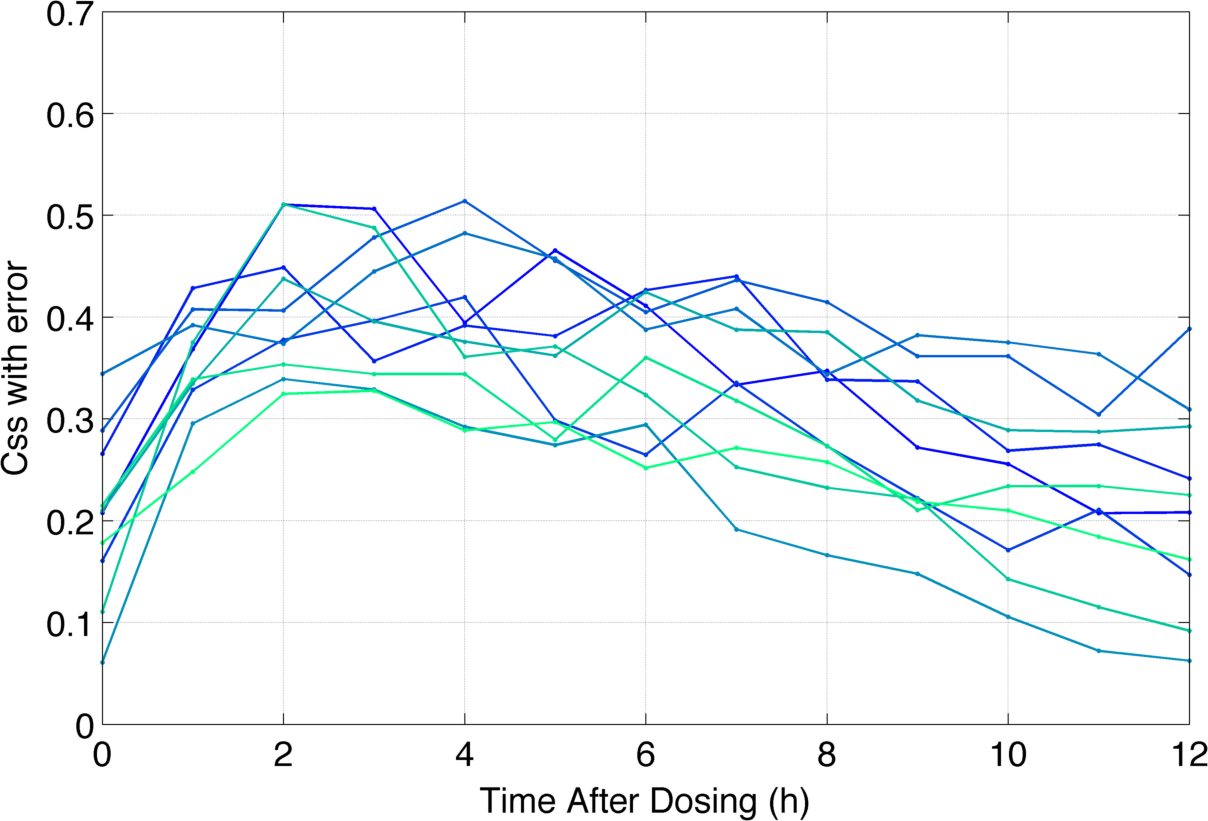
\includegraphics[width=.45\textwidth]{pics/Bonate_Css_proportionalError}
\caption{Simulated PK model as defined in the example for 10 subjects.}
\label{fig:BonatePK}
\vspace{-20pt}
\end{center}
\end{figure}
The only essential new aspect compared to the previous example is the fact
that we have here so called steady-state administration. For this to be defined
one needs to provide the time point of the last dosing event and the dose interval.

\subsubsection{Variability model}
The variability structure is identical to that in the previous example -- there is only
one level of subject related variability, see Figure \ref{fig:tree_IOV0}.

\subsubsection{Parameter model}

The model uses the following parameters:

\begin{align*}
\theta_{1,i} &=  \pop_{\theta_1} + \eta_{\theta_1,i}   \\
\log(V_i) &= \log(\pop_{V}) + \eta_{V,i}   \\
\theta_2 &= 0.75 \\
CL_i &= \theta_{1,i} \Big(\frac{W_i}{70}\Big)^{\theta_2} \\
K_a &= 0.5
\end{align*}
where
\begin{gather*}
\eta_{\theta_{1,i}} \sim N(0, \omega_{\theta_1}), \quad \eta_{V,i} \sim N(0,\omega_{V})
\intertext{and with}
\pop_{\theta_1}=25,\quad \omega_{\theta_1}=5  \quad \pop_V=250,\quad \omega_V=100.
\end{gather*}

\subsubsection{Covariate model}
%\begin{align*}
%\Covariates &: \Weight/70  \\
%\CovariatesType &: \Continuous  \\
%\CovariatesFile &: e.g. \textit{some\_filename.txt}  \\
%\Weight &\sim  \mbox{logNormal}(pop_{\Weight}, \omega_{\Weight}); \quad \pop_{\Weight}=80,\quad \omega_{\Weight}=9.6 
%\end{align*}

Body weight is the only covariate used in this model. It is used in the model
for the individual clearance only.
\begin{table}[h]
\begin{center}
\begin{tabular}{lr}\toprule
 & \textbf{Weight} \\\midrule
Type & Continues \\
Transformation & $(\Weight/70)^{\theta_2}$ \\
Distribution & Normal \\
Mean, $pop_{\Weight}$ & 80 \\
Standard deviation, $\omega_{\Weight}$ & 9.6 \\
\bottomrule
\end{tabular}
\end{center}
\caption{Covariates overview.}
\label{tab:CovariatesOverview}
\end{table}


\subsubsection{Structural model}
\begin{align*}
k &= \frac{CL}{V} \\
C_{SS}(t) &= \frac{D}{V}\frac{K_a}{K_a - k} \bigg(\frac{e^{-k (t-t_D)}}{1-e^{-k \tau}}-\frac{e^{-K_a (t-t_D)}}{1-e^{-K_a\tau}}\bigg) 
\end{align*}

\subsubsection{Observation model}

We apply a residual error models to the output variable \var{C_{SS}}.

%\noindent
\begin{center}
\begin{tabular*}{0.6\textwidth}{@{\extracolsep{\fill}} >{\bfseries}l l}\toprule
Output Variable  & \textbf{\itshape $C_{SS}$} \\\midrule
Observations Name & Concentration\\
Units & $\mg/l$ \\
Observations Type & Continuous \\
Residual Error Model & Proportional \\
Error Model Parameters & $b=0.1$\\
\bottomrule
\end{tabular*}
\end{center}

%%%%%%%%%%%%%%%%%%%%%%%%%%%%%%%%%%%%%%%%%%%%%%%%%%%%%%%%%%%%%%%%
\subsubsection{Trial design}

Table below summarises the information about the design in this example. 

%\noindent
\begin{center}
\begin{tabular*}{0.45\textwidth}{@{\extracolsep{\fill}} >{\bfseries}l r}\toprule
Arm & \textbf{1} \\\midrule
Number of subjects & 50\\
Dose variable & \var{D} \\
Dosing Amount & 100 \\
Dose Units & $\mg$  \\
Dose per kg & no \\
Dosing times (h) & 0\\
Dose intervals (h) & 12\\
\bottomrule
\end{tabular*}
\end{center}

%%%%%%%%%%%%%%%%%%%%%%%%%%%%%%%%%%%%%%%%%%%%%%%%%%%%%%%%%%%%%%%%
\subsubsection{Simulation Step}
The concentration $C_{SS}$ is going to be read out at equidistant time points
after the dosing:
\begin{center}
\begin{tabular*}{0.6\linewidth}{@{\extracolsep{\fill}} >{\bfseries}l c}\toprule
Output Variable & \textbf{\itshape $C_{SS}$}\\
Observation times & 0,1,2,3,4,5,6,7,8,9,10,11,12\\
\bottomrule
\end{tabular*}
\end{center}

\subsection{Structural model}
In the last example we defined the structural model by using an ODE system. 
Here, we implement an algebraic formula for the calculation of the drug
concentration in steady-state, \var{C_{SS}}, as shown in the following listing
\inputxml{bonate_sm1_part1.xml}
Consequently, we use for \var{C_{SS}} the \xelem{Variable}, instead of \xelem{DerivativeVariable},
element as in the previous example which is of \xatt{real} type.

\subsection{Trial design model}
\subsubsection{Structure}

Figure \ref{fig:designPatternBonate} shows the \textit{Structure} of
this simple example consisting of 1 arm and one epoch, meaning one treatment
type for everybody.

\begin{figure}[ht!]
\centering
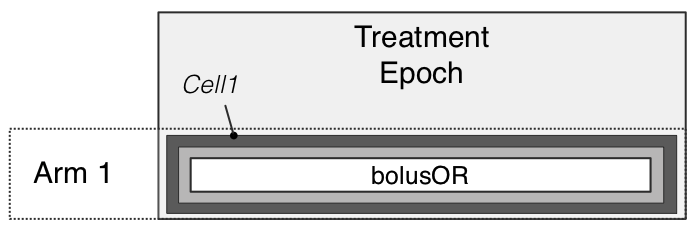
\includegraphics[width=0.7\linewidth]{../pics/OneArmOneEpoch_Bonate}
\caption{Design overview: this study consists of one arm and one epoch.}
\label{fig:designPatternBonate}
\end{figure}

\begin{table}[htdp!]
\begin{center}
\begin{tabular}{ccccccc}
\hline
Segment&Activity & Treatment & DoseTime & DoseSize & Target Variable \\
\hline
TA& bolusOR &  OR bolus & 0 & 100 & D \\
\hline
\end{tabular}
\end{center}
\caption{Segment/activity overview.}
\label{tab:segementActivity_Ribba}
\end{table}

\begin{table}[htdp!]
\begin{center}
\begin{tabular}{ccc}
\hline
Epoch & Start time & End time \\
\hline
Treatment Epoch & 0 &  12  \\
\hline
\end{tabular}
\end{center}
\caption{Epoch definition -- there is only one epoch here.}
\label{fig:Bonate:epochDef}
\end{table}

While the implementation of epoch, arm, cell and segment is analog to that in the 
previous example, the \xelem{Activity} element contains new items. After we 
defined \xelem{DoseAmount} as before as well, the steady-state administration 
is easily implemented using the \xelem{SteadyState} with last doing event as
\xelem{EndTime} and the dose interval as \xelem{Interval} as can be seen 
in the following listing \inputxml{bonate_activity.xml}



%%%%%%%%%%%%%%%%%%%%%%%%%%%%%%%%%%%%%%%%%%%%%%%%%%%%%%%%%%%%%%%%
%%%%%%%%%%%%%%%%%%%%%%%%%%%%%%%%%%%%%%%%%%%%%%%%%%%%%%%%%%%%%%%%
%%%%%%%%%%%%%%%%%%%%%%%%%%%%%%%%%%%%%%%%%%%%%%%%%%%%%%%%%%%%%%%%
\eglabel{4}
\section{Example \theexamples: Estimation, Warfarin PK}
\label{sec:eg4}

\subsection{Description}

This model describes the PK of the drug Warfarin and corresponds to
the \ddmore WP3 use case Warfarin\_PK\_PRED\footnote{\raggedright Available via Interface Europe: \url{https://cp1.interfaceurope.eu/LotusQuickr/ddmore/PageLibraryC125786900388659.nsf/h_Toc/92be13faec1b58390525670800167238/?OpenDocument\#{type=0\&unid=5801C48FC6C39BB141257B2A007D6F31}}}. 

\subsubsection{Structural model}

The model is a one compartment model with first-order absorption with
lag time and first-order elimination.

\begin{description}
\item[\itshape D] Dosing variable.
\item[\itshape t\textsubscript{D}] Time of the dose.
\item[\itshape C] Concentration of drug in the compartment.
\end{description}
\begin{align*}
k &= \frac{\CL}{V}\\
C(t) &= \begin{cases}
  0 & \text{if } \quad t - t_D < \Tlag \\
  \frac{D}{V}\frac{k_a}{k_a-k}\left[e^{-k\,
       \left(t-t_D-T_{lag}\right)}-e^{-k_a \, \left(t-t_D-T_{lag}\right)}\right] &
  \text{otherwise}
\end{cases}
\end{align*}


\subsubsection{Covariate model}

%The covariate is Weight, $W$, a continuous covariate with the following transformation applied:
%\begin{gather}
%%W \sim \mathcal{N}(\pop_{\Weight}, \omega_{\Weight})
%\log(\Weight/70) \nonumber
%%\intertext{initial values:}
%%\pop_{\Weight} =70.07, \quad \omega_{\Weight} =14.09 \nonumber
%\end{gather}
%
Body weight, $W$, is the only continue covariate used in this model. It is used in the model
for the individual clearance and volume.
\begin{table}[h]
\begin{center}
\begin{tabular}{lr}\toprule
 & \textbf{Weight} \\\midrule
Type & Continues \\
Transformation & $\log(\Weight/70)$ \\
\bottomrule
\end{tabular}
\end{center}
\caption{Covariates overview.}
\label{tab:CovariatesOverview}
\end{table}




\subsubsection{Parameters}

\paragraph{PK Parameters}

The following PK parameters are used in the model:
\begin{description}
\item[\Tlag] The lag time.
\item[\ka] The absorption rate constant.
\item[\var{V}] The volume of distribution.
\item[\CL] Clearance of elimination.
\end{description}

\begin{align*}
\intertext{The parameters are defined as follows:}
\log(\Tlag) &= \log(pop\_\Tlag) + \eta_\Tlag\\
\log(\ka) &= \log(pop\_\ka) + \eta_\ka\\
\log(\var{V}) &= \log(pop\_\var{V}) + \beta_{1,V} \log(W_i/70) + \eta_\var{V}\\
\log(\CL) &= \log(pop\_\CL) + \beta_{1,\CL} \log(W_i/70) + \eta_\CL
\end{align*}
where
\begin{gather*}
\eta_\Tlag \sim \mathcal{N}(0, \omega_{\Tlag}), \quad \eta_\ka \sim \mathcal{N}(0, \omega_{\ka}),\\
\eta_\var{V} \sim  \mathcal{N}(0, \omega_{V}), \quad \eta_\CL \sim \mathcal{N}(0, \omega_{\CL})
\end{gather*}
Note please that, in this case, $\beta_{1,V}=0.75$ and $\beta_{1,CL}=1$, i.e. are fixed and will not be estimated.

\paragraph{Variance-covariance matrix}
The full variance-covariance matrix for the random effects is :
\begin{equation*}
 \Omega =
 \begin{pmatrix}
  \omega_{Tlag}^2 	& 0 				& 0                                 & 0  \\
   			  	& \omega_{\ka}^2	& 0                                 & 0  \\
  				& 				& \omega_{\var{V}}^2     & 0  \\
 				&				&                                    & \omega_{\CL}^2 \\
 \end{pmatrix}
%\label{sec:eg-covariance-mat}
\end{equation*}

\subsubsection{Observation model}

We apply a residual error models to the output variable \var{C}.

%\noindent
\begin{center}
\begin{tabular*}{0.6\textwidth}{@{\extracolsep{\fill}} >{\bfseries}l l}\toprule
Output Variable  & \textbf{\itshape C} \\\midrule
Observations Name & Concentration\\
Units & $\mg/l$ \\
Observations Type & Continuous \\
Residual Error Model & Combined2 \\
Error Model Parameters & $a = 0.1,\quad b=0.1$\\
\bottomrule
\end{tabular*}
\end{center}

\subsubsection{Trial Design}
\label{sec:eg4-trial-design}

The dosing regimen for the trial is given below --- there is only one
for each arm. Note that all dosing is bolus dosing (discrete
administration at specific times) and all doses are administered to
the same compartment.

%\noindent
\begin{center}
\begin{tabular*}{0.45\textwidth}{@{\extracolsep{\fill}} >{\bfseries}l r}\toprule
Arm & \textbf{1} \\\midrule
Number of subjects & 33\\
Dose variable & \var{D} \\
Dosing Amount & 100 \\
Dose Units & $\mg$  \\
Dose per kg & no \\
Dosing times (h) & 0\\
\bottomrule
\end{tabular*}
\end{center}

% The trial is has just one study group of 33 individuals.
% \begin{align*}
% \DoseTime (t_D)&= 0    \\
% \TimeUnit&= h
% \intertext{Dosing is adjusted to body weight}
% \DoseSize&= 100  \\
% \DosePerKg&=\no   \\
% \DoseUnit&=\mg
% \intertext{Time of measurement for PK}
% \ObservationTime&= 0.5,1,2,3,6,9,24,36,48,72,96,120
% \end{align*}

\subsubsection{Modelling Steps}

The observations for the output variable is shown below. These
time-points correspond to those define in the data-file. The task to
be performed is a parameter estimation which will involved the
following steps:
\begin{itemize}
\item Estimation of population paramaters.
\item Estimation of Fisher information matrix.
\item Estimation of the individual parameters.
\end{itemize}

%\noindent
\begin{center}
\begin{tabular*}{0.6\linewidth}{@{\extracolsep{\fill}} >{\bfseries}l c}\toprule
Output Variable & \textbf{\itshape C}\\
Observation times & 0.5,1,2,3,6,9,24,36,48,72,96,120\\
\bottomrule
\end{tabular*}
\end{center}

\begin{figure}[ht!]
\centering
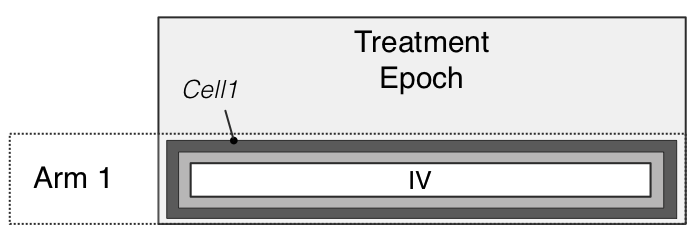
\includegraphics[width=0.7\linewidth]{../pics/designPattern_1Arm1Epoch}
\caption{Design overview: this study consists of one arm and one epoch.}
\label{fig:designPattern_1Arm1Epoch}
\end{figure}

Figure \ref{fig:designPattern_1Arm1Epoch} shows the \textit{Structure} of
this simple example consisting of 1 arm and one epoch, meaning one treatment
type for everybody.

%
% The output variable is:
% \begin{description}
% \item[\var{C}] Concentration in the central compartment, in this case
%     the bloodstream.
% \end{description}

\subsection{Overview}

This our first estimation case. From figure \ref{fig:simEstTasks_List} 
it follows that we can expect significant differences in the Trial Design and Modelling Steps
sections compared to the previous simulation case.

%, see listing \ref{fig:exp5_modelOverview}
%for an overview.

Accordingly, the Model Definition is very similar to that in the
previous example.  The main \pharmml feature we have not seen
previously is the algebraic structural model (i.e., the model is not
defined as a system of ODEs). The XML is too long to show here and is
similar to the examples shown previously (section \ref{sec:maths}). If
you are interested then please consult the full example associated
with this specification.

We will start with the description of the Trail design. Note that because
every subject receives the same dosing regimen, this can be encoded 
in the \xelem{Activity} block. Otherwise we would have to define the 
individual dosing regimens in the \xelem{IndividualDosing} element, see
section \ref{subsubsec:Ribba_indivDosing} in example \ref{sec:Ribba} how
this is done.

%\begin{listing}[htb]
%\inputxml{exp5_modelOverview.xml}
%\caption{Defining the complete model.}
%\label{fig:exp5_modelOverview}
%\end{listing}


\subsection{Trial Design}
\label{eg4_subsec:trialDesign}
\subsubsection{Structure}

As explained in the chapter \ref{sec:CTS} on trial design, we base the following 
structure on the CDISC standard Study Design Model \cite{CDISC:2011a}. 
The design elements are contained in the \xelem{Structure} block and you can see 
in following listing \inputxml{exp5_structure.xml}
how the study is constructed of a single epoch, 
with a single arm and a single cell that contains a single segment. Note, though 
that this structure is not hierarchical and the \xelem{Cell} element joins the arm, 
epoch and segments together. 

The last section of the structure, the \xelem{Activity} element, is of interest for 
the discussion. This is because, as already mentioned above, the administration
and dosing regimen is identical for every patient. The dose amount is $D=100\; mg$ 
and the dose time is $t_D=0$.
As in the previous example, the structural model is defined using an algebraic
function with the dosing variable \var{D} which means the \xelem{DoseAmount} element
has the attribute \xatt{inputType="dose"}. Additionally the dosing time variable \var{tD} is
referenced here and initialised. 


%\begin{listing}[htb]
%\inputxml{exp5_structure.xml}
%\caption{Structure overview.}
%\label{lst:exp5_structure}
%\end{listing}

\subsubsection{Population}

This is the place where we describe the individuals in the study, which 
\var{Arm} they belong to and any possible individual characteristics, such as 
body weight, age and other covariates. In this example we only know the
body weight of the subjects. 
We define the known attributes of all individuals using the 
\xelem{IndividualTemplate} and then map each individual to this template 
using a \xelem{Dataset}. In the following listing \inputxml{exp5_population.xml}
you can see how this 
is implemented in \pharmml. Column \var{2} in the table is equal for
every subject because they all belong to one arm, here denoted as \var{a1}.

%\begin{listing}[htb]
%\inputxml{exp5_population.xml}
%\caption{Population overview.}
%\label{fig:exp5_population}
%\end{listing}

\subsection{Modelling Steps}

\subsubsection{Objective data}

The biggest advantage of the current specification is that we do not have
to define the design in the data file. After the structure of the trial is defined
as above we just need to encode the measured experimental data, here the time 
and the independent variable, the concentration values. To achieve that we 
define a table in \xelem{Dataset} with columns: \var{ID}, \var{time} and 
\var{dv} and populate it with given experimental values, see \xelem{ObjectiveDataSet} block 
in the following listing \inputxml{exp5_objDataSet.xml}
Before that we have to make sure that these values are correctly mapped to 
variable used in the model which is implemented in the \xelem{VariableMapping}
element. Accordingly, we define the identifier \var{ID} and 
define the variable mapping. Here the \var{time} as in the data is mapped 
to model time \var{t} and the measured concentration is mapped to the 
variable \var{C} as in the observation model.


%\begin{listing}[htb]
%\inputxml{exp5_objDataSet.xml}
%\caption{Objective dataset overview.}
%\label{fig:exp5_objDataSet}
%\end{listing}	

\subsubsection{Parameter estimation}


In a parameter estimation you do not necessarily want to estimate all
the parameters in your model or you may wish to define bounds within
which your parameter should be estimated, or provide an initial
estimate.  The \xelem{ParametersToEstimate} element controls this. As
you can see in the following listing \inputxml{exp5_paramEstimation.xml}
we use a \xelem{ParameterEstimation} element that refers to the parameter in
the model definition.  In its simplest form you can decide whether the
parameter is to be estimated by setting the \xatt{fixed} attribute
(false indicates the parameter should be estimated). If a parameter is
not defined here, then it is assumed that it will not be estimated, in
which case it would be assigned an initial value elsewhere in the
PharmML document.  One of the validation rules (see chapter
\ref{chapter:validation}) is that every parameter has to be
initialised. 
%This can happen either in the \xelem{ParameterModel},
%\xelem{ObservationModel} or in this \xelem{ParametersToEstimate} block.
 

%\subsubsection{Operation}
%
%\begin{listing}[htb]
%\inputxml{exp5_operation.xml}
%\caption{Operation overview.}
%\label{fig:exp5_operation}
%\end{listing}


\subsubsection{Step dependencies}

Then at the end of the \xelem{ModellingSteps} block is the \xelem{StepDependencies} element. 
This describes the ordering of the steps in the modelling process, but in this case it is 
almost trivial as we only have one step in this example:
\inputxml{exp5_steps.xml}


%\begin{listing}[htb]
%\inputxml{exp5_steps.xml}
%\caption{Step dependencies overview.}
%\label{fig:exp5_steps}
%\end{listing}






%%%%%%%%%%%%%%%%%%%%%%%%%%%%%%%%%%%%%%%%%%%%%%%%%%%%%%%%%%%%%%%%
%%%%%%%%%%%%%%%%%%%%%%%%%%%%%%%%%%%%%%%%%%%%%%%%%%%%%%%%%%%%%%%%
%%%%%%%%%%%%%%%%%%%%%%%%%%%%%%%%%%%%%%%%%%%%%%%%%%%%%%%%%%%%%%%%
\eglabel{6}
\section{Example \theexamples: Estimation with IOV}
\label{sec:eg6}

%%%%%%%%%%%%%%%%%%%%%%%%%%%%%%%%%%%%%%%%%%%%%%%%%%%%%%%%%%%%%%%%
\subsection{Description}

In this example we will look at more complex trial design and a
correspondingly complex variability model. The model also includes
categorical covariates, which is again something we have not
encountered thus far. The example is based on example IOV1 from
Monolix 4.1 (see \cite{Monolix4.1.4UserGuide:2012} for a detailed
description) and features a cross-over design and inter-occasion
variability (see section \ref{sec:variabilityModel}). As before we will
go through the key elements of the model before we look at the
\pharmml examples, but given the complex nature of the trial design we
will describe that first then move onto the model definition.


\begin{figure}[htb]
\centering
 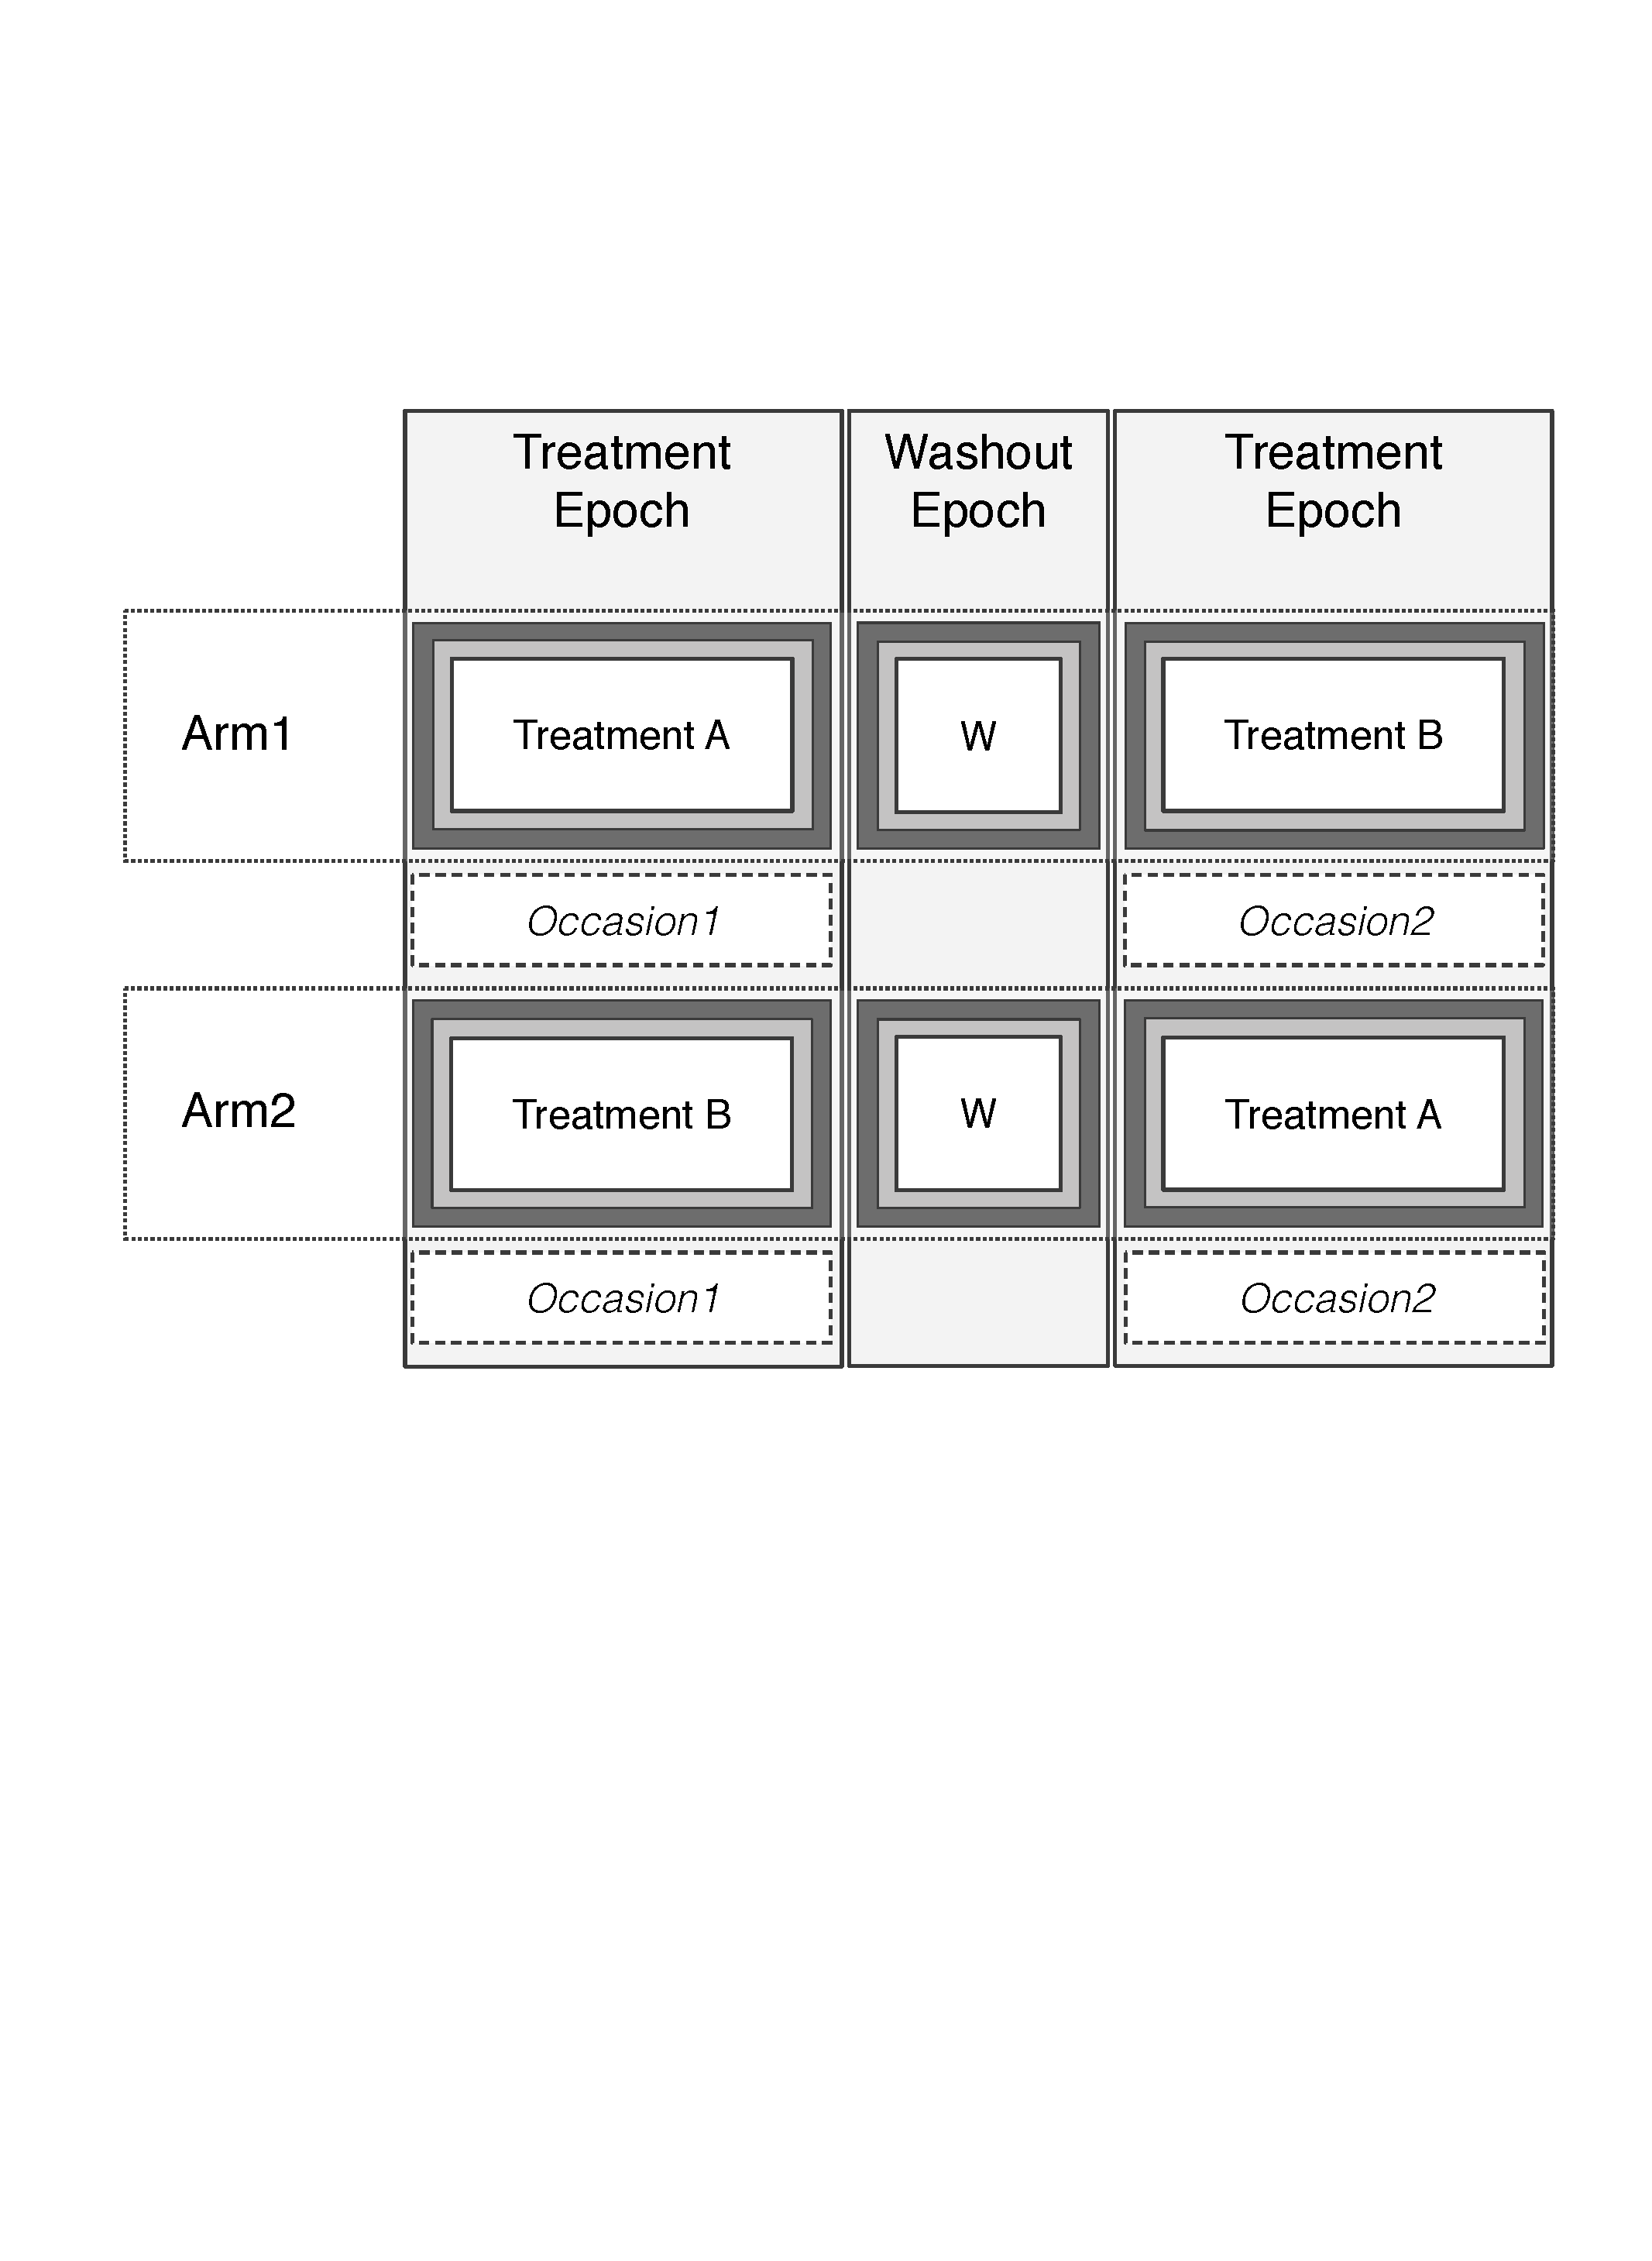
\includegraphics[width=0.7\linewidth]{TwoArmsThreeEpochs_withWashout.pdf}
\caption{Schematic representation of a crossover design with washout. The reader is referred to
Figure \ref{fig:templateTrialDesign} for the colour code used to identify the elements of
a trial. See tables \ref{fig:eg6:segmentCellArmEpoch} 
and \ref{fig:eg6:epochDef} for the detailed definition of segments, cells, arms, epochs
and occasions in this example.}
\label{fig:TwoArmsThreeEpochs_withWashout}
\end{figure}

%\noindent
\begin{table}[h]
\begin{center}
\begin{tabular}{lrr}\toprule
Arm & \textbf{1} & \textbf{2} \\\midrule
Number of subjects & 33 & 33\\
Dose variable & \var{D} & \var{D} \\
Dosing Amount & 100 & 150 \\
Dose Units & $\mg$ & $\mg$  \\
Dose per kg & no & no \\
Dosing times (h) &  [0 : 12 : 72] &  [0 : 12 : 72\\
\bottomrule
\end{tabular}
\end{center}
\caption{Arms overview with dosing specification.}
\label{tab:ArmOverview}
\end{table}


%%%%%%%%%%%%%%%%%%%%%%%%%%%%%%%%%%%%%%%%%%%%%%%%%%%%%%%%%%%%%%%%
\subsubsection{Trial Design}
The model features a basic crossover design (see Figure
\ref{fig:TwoArmsThreeEpochs_withWashout}) with washout period and inter-occasion
variability (IOV). There are two treatments and the subjects are
organised into two arms that start with a different treatment. In
between each treatment there is a washout period during which time the
drug is eliminated from each subject. 
In the model the treatments, fi treated as occasions, provide a second level of variability -- 
IOV \index{variability!IOV} (see section \ref{sec:variabilityModel}).  
This is summarised in Figure \ref{fig:eg6-IOV_2levels} (see also the listing 
in section \ref{eg6:variabilityModel}, showing relevant code 
within the element \xelem{VariabilityModel}).

The model also uses covariates to model the variability within the
model and so the treatments, the sequence of treatments (i.e.\xspace treatments A, B or
B,A) and the occasion itself are described in the covariate section
below.

\begin{figure}[ht!]
\centering
 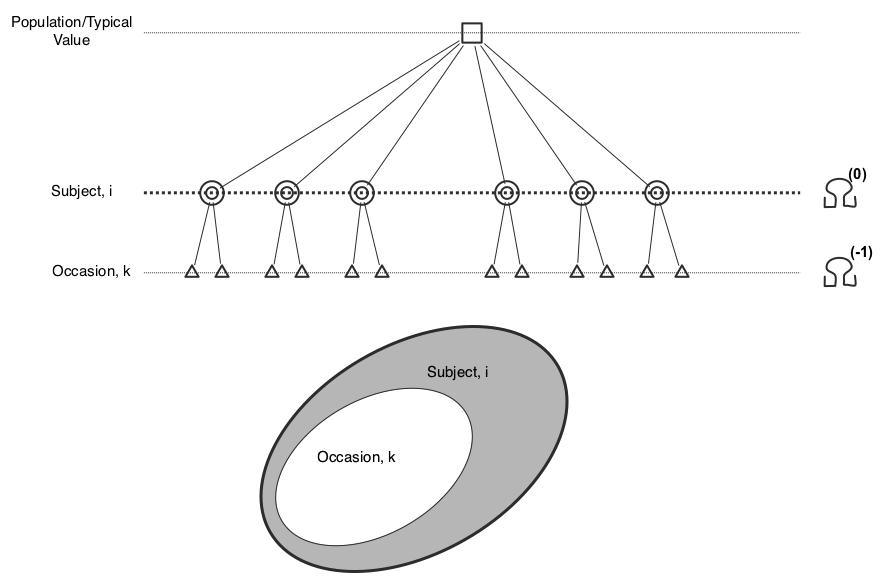
\includegraphics[width=120mm]{IOV_2levels}
\caption{Two levels of variability -- inter-individual and inter-occasion within individual variability.}
\label{fig:eg6-IOV_2levels}
\end{figure}


%%%%%%%%%%%%%%%%%%%%%%%%%%%%%%%%%%%%%%%%%%%%%%%%%%%%%%%%%%%%%%%%
\subsubsection{Covariate Model}
\label{eg6:covariates-defn}

As discussed about all but the `Sex' covariate is used to capture the
variability in the model, see Table \ref{tab:CovariatesOverview}.

\begin{table}[h]
\begin{center}
\begin{tabular}{lrrrr}\toprule
 & \textbf{Sex} &{\color{red}\textbf{Treat}}&{\color{mediumgreen}\textbf{TreatSeq}}&{\color{magenta}\textbf{Occasion}}\\\midrule
Type & Categorical & Categorical & Categorical & Categorical  \\
Category Count & 2 & 2 & 2 & 2\\
Categories & F, M & A, B & A--B,B--A & 1, 2\\
Reference & F & A & A--B & 1\\
%Reference Probability & $14/36$ & 0.5  & 0.5  & 0.5\\
\bottomrule
\end{tabular}
\end{center}
\caption{Covariates overview.}
\label{tab:CovariatesOverview}
\end{table}

%%%%%%%%%%%%%%%%%%%%%%%%%%%%%%%%%%%%%%%%%%%%%%%%%%%%%%%%%%%%%%%%
\subsubsection{Parameter Model}

The parameter model includes random effects that represent the IIV and
{\color{lightblue}IOV} levels of variability. It also relates the
parameters to the covariates described above\footnote{To improve
  clarity we have colour coded the contributions of the different levels
of variability and the different covariates.}

\begin{align}
\log(ka_{i}) &= \log(ka_{pop}) +
{\color{mediumgreen}\beta_{ka,TreatSeq}}1_{TreatSeq_i=A-B} +
\eta_{ka,i} \label{eqn:eg6-param-ka}\\
\begin{split}
\log(V_{ik}) &= \log(V_{pop}) + {\boldsymbol \beta_V}1_{S_i=F} +
{\color{magenta}\beta_{V,OCC}} 1_{OCC_{ik}=1} \\
&\quad+ {\color{red}\beta_{V,Treat}}1_{Treat_{ik}=A} + {\color{mediumgreen}\beta_{V,TreatSeq}}1_{TreatSeq_i=A-B} \\
		& \quad+ \eta_{V,i}^{(0)} +  {\color{lightblue} \eta_{V,ik}^{(-1)} }
\end{split} \label{eqn:eg6-parameter-v}\\
\begin{split}
\log(\CL_{ik}) &= \log(\CL_{pop}) + {\boldsymbol \beta_{\CL}}1_{S_i=F}
+ {\color{magenta}\beta_{\CL,OCC}} 1_{OCC_{ik}=1}\\
&\quad + \eta_{\CL,i}^{(0)} + {\color{lightblue} \eta_{Cl,ik}^{(-1)} }
\end{split}\nonumber
\end{align}
where
\begin{gather*}
\eta_{ka,i}^{(0)} \sim \mathcal{N}(0, \omega_{ka}), \quad \eta_{V,i}^{(0)} \sim \mathcal{N}(0, \omega_{V}), \quad \eta_{\CL,i}^{(0)} \sim \mathcal{N}(0, \omega_{\CL}),  \\
 {\color{lightblue} \eta_{V,ik}^{(-1)} \sim \mathcal{N}(0,\gamma_V)}, \quad
 {\color{lightblue} \eta_{\CL,ik}^{(-1)} \sim \mathcal{N}(0, \gamma_{\CL})}
\end{gather*}

The full variance-covariance matrix for our model is :
\begin{gather}
 \Omega^{(0)} =
 \begin{pmatrix}
  \omega_{ka}^2 	& 0 				& 0  \\
   			  	& \omega_{V}^2	& 0 	\\
  				& 				& \omega_{\CL}^2\\
 \end{pmatrix}\label{eqn:eg6-covariance-mat}\\
 \Omega^{(-1)} =
 \begin{pmatrix}
0 & 0 & 0\\
 & \gamma_{V}^2	& 0 	\\
 & & \gamma_{\CL}^2\\
 \end{pmatrix}\label{eqn:eg6-gamma-mat}
\end{gather}


%%%%%%%%%%%%%%%%%%%%%%%%%%%%%%%%%%%%%%%%%%%%%%%%%%%%%%%%%%%%%%%%
\subsubsection{Structural model}

The model is first order absorption with linear elimination, with
multiple dosing. This is the equivalent to oral1\_1cpt\_kaVCl (model 8) from \cite[Appendix I]{Bertrand:2008}.


%%%%%%%%%%%%%%%%%%%%%%%%%%%%%%%%%%%%%%%%%%%%%%%%%%%%%%%%%%%%%%%%
\subsubsection{Observation model}

We apply a residual error models to the output variable \var{C}.

%\noindent
\begin{center}
\begin{tabular*}{0.6\textwidth}{@{\extracolsep{\fill}} >{\bfseries}l l}\toprule
Output Variable  & \textbf{\itshape C} \\\midrule
Observations Name & Concentration\\
Units & $\mg/l$ \\
Observations Type & Continuous \\
Residual Error Model & Combined \\
Error Model Parameters & $a = 0.1,\quad b=0.1$\\
\bottomrule
\end{tabular*}
\end{center}


%%%%%%%%%%%%%%%%%%%%%%%%%%%%%%%%%%%%%%%%%%%%%%%%%%%%%%%%%%%%%%%%
\subsubsection{Modelling Steps}
Compared to the last example, we have define here two tasks:
\begin{itemize}
\item Estimation of population paramaters.
\item Estimation of the individual parameters.
\end{itemize}

%%%%%%%%%%%%%%%%%%%%%%%%%%%%%%%%%%%%%%%%%%%%%%%%%%%%%%%%%%%%%%%%
\subsection{Trial Design}

We have summaries the dosing regimen and organisation of the trial
design below, see also Figure \ref{fig:TwoArmsThreeEpochs_withWashout}.

\begin{table}[htdp!]
\begin{center}
\begin{tabular}{ccccccc}
\hline
Segment&Activity & Treatment & DoseTime & DoseSize & Target Variable \\
\hline
TA& OR1 &  OR bolus & $0:12:72$ & 150 & Ac \\
TA& OR2 &  OR bolus & $0:24:72$ & 100 & Ac \\
\hline
\end{tabular}
\end{center}
\caption{Segment/activity overview.}
\label{fig:eg6:segmentCellArmEpoch}
\end{table}

\begin{table}[htdp!]
\begin{center}
\begin{tabular}{cccc}
\hline
Epoch & Occasion & Start time & End time \\
\hline
Treatment Epoch & OCC1 & 0 &  180  \\
Washout & -- & 0 &  10  \\
Treatment Epoch & OCC2 & 0 &  180  \\
\hline
\end{tabular}
\end{center}
\caption{Epoch and occasion definition.}
\label{fig:eg6:epochDef}
\end{table}


%%%%%%%%%%%%%%%%%%%%%%%%%%%%%%%%%%%%%%%%%%%%%%%%%%%%%%%%%%%%%%%%
\subsubsection{Structure}
The implementation of the treatments, in \pharmml we use the
\xelem{Activity} element, is different compared to the previous example. 
See Table \ref{fig:eg6:segmentCellArmEpoch} for the details. The difference
is that now we have one dose administered at multiple dosing time points 
instead of single time point. See the following listing \inputxml{exp6_dosingTimes.xml}
how one can describe it within the \xelem{DosingTimes} element using the \xelem{Sequence}
structure defining the start/end times and step size.

Table \ref{fig:eg6:epochDef} gives an overview of the \var{Epochs} and \var{Occasions} 
in this example. Here, the occasions overlap with the epochs, the start and end times 
are identical, this is not always the case, the occasions can span one or more epochs. 
The \var{Washout} epoch is given here with start/end times as well which is in fact 
a redundant piece of information (but required by construction of an \var{Epoch})
as a \var{Washout} always assumes total reset of all drug amounts. 

%\begin{listing}[ht!]
%\inputxml{exp6_structure_part3.xml}
%\caption{The implementation of the mapping of IOV to the trial design.}
%\label{exp6_structure_part3}
%\end{listing}

As discussed in the section \ref{subsec:TrialStructure}, in \xelem{Structure} block 
we encode the variability which is located below the subject (see the 
hierarchy of the random variability discussed in section \ref{sec:variabilityModel}).
We call it the \textit{inter-occasion variability}, IOV. The following listing 
\inputxml{exp6_structure_part3.xml} shows how this is done. 
In this case the occasions coincide with the epochs 
so we use the \xelem{EpochRef} element. Alternatively, we could use the \xelem{Period}
element to define explicitly the start and end times of the occasions as shown 
in this listing: \inputxml{exp6_structure_part4.xml}
This is of course very useful if the occasions do not
coincide with the epochs, or there are two or more occasions within one epoch.
In this case we set the \var{Start} and \var{End} times to $0$ and $180$, respectively.
These are exactly the same time points as are used in the epoch definition 
(see the first listing in section \ref{eg4_subsec:trialDesign} for how to encode epochs in the 
\xelem{Structure} definition).   

%\begin{listing}[ht!]
%\inputxml{exp6_structure_part4.xml}
%\caption{Alternative implementation of the mapping of IOV to the trial design shown in previous listing.}
%\label{exp6_structure_part4}
%\end{listing}
 

%%%%%%%%%%%%%%%%%%%%%%%%%%%%%%%%%%%%%%%%%%%%%%%%%%%%%%%%%%%%%%%%
\subsubsection{Population}
We pick up where we left off in the \xelem{Structure}, implementing
the hooks to the variability structure. The aspect we have not covered
yet is related to IIV.  The \xelem{Population} element is the place to
define any subject related variability and those levels above
it. The following listing shows how this works \inputxml{exp6_population_part0.xml}
Here we deal only with the IIV so we are done with this aspect.

%\begin{listing}[ht!]
%\inputxml{exp6_population_part0.xml}
%\caption{The implementation of the IIV mapping.}
%\label{exp6_population_part0}
%\end{listing}

The next part of the \xelem{Population} block was discussed previously, 
with one exception. Beside the standard assignment of subjects to an \var{Arm}
and providing information regarding \var{Sex}, we need to encode the information
about \var{Treat}, i.e. treatment type considered here as covariate, which varies
by definition in this cross-over design as the study progress from \var{Epoch1}
to \var{Epoch3}. To encode this we use the \textit{nested table} concept as described 
in section \ref{sec:dataset}. 
Here the child table is defined by using a \xelem{Table} element instead of the 
usual \xelem{Column} element and given the identifier 'treat-tab'. 
Within the nested table definition another set of relevant columns is specified, 
\var{epoch} and \var{treat}. Next these nested tables are populated with 
data as can be seen in the following listing \inputxml{exp6_population_part2.xml}
here for \var{Arm1}.
Listing \inputxml{exp6_population_part2B.xml}
shows one data record for \var{Arm2}.

%\begin{listing}[ht!]
%\inputxml{exp6_population_part2.xml}
%\caption{The implementation of the nested table for time varying covariate, \var{Treat}, for  \var{Arm1}.}
%\label{exp6_population_part2}
%\end{listing}

%\begin{listing}[ht!]
%\inputxml{exp6_population_part2B.xml}
%\caption{The implementation of the nested table for time varying covariate, \var{Treat},  for  \var{Arm2}.}
%\label{exp6_population_part2B}
%\end{listing}


%%%%%%%%%%%%%%%%%%%%%%%%%%%%%%%%%%%%%%%%%%%%%%%%%%%%%%%%%%%%%%%%
\subsection{Variability Model}
\label{eg6:variabilityModel}

In this example the variability model is more complex than before, with IIV\index{variability!IIV} and IOV\index{variability!IOV} levels of variability, see Figure \ref{fig:eg6-IOV_2levels}. As you will see, in \pharmml the complexity comes later -- in the parameter model. At this point in the \pharmml document all we need to do is define the variability levels to be used in the rest of the document. You can see in the following listing \inputxml{exp6_iov.xml}
that this is done simply by listing the variability levels using the \xelem{VariabilityLevel} element. There are three important points to note here:
\begin{enumerate}
\item There is parent-child relationship between the levels of variability. The \var{Subject} level, 
in the \pharmml it is referenced with the attribute \xatt{symbId="indiv"} is higher
in the hierarchy and directly above the \var{Occasion} level, referenced with the 
attribute \xatt{symbId="iov1"} which is exactly what is done
using the \xelem{ParentLevel} in the listing above.
\item The name given to a level, using the \xatt{symbId} attribute, is \textbf{not} significant. We used the names \var{iov1} and \var{indiv} to provide clarity in other parts of the example document.
\item the type of each variability level (e.g.,\xspace between-subject, inter-occasion, between-centre) is not defined here or in the Model Definition as a whole\footnote{N.B.,\xspace The numerical levels described in the variability model (section \ref{sec:variabilityModel}) are not used.}.
\end{enumerate}

So in this example the \pharmml document tells us that there are two variability levels and that the lowest level of variability is called ``\texttt{iov1}''\index{variability!IOV}\@. This may seem odd, but to simulate or estimate the model we do not need to know which level of variability is considered IIV and which IOV.  We only need to know their level relative to each other. Of course it may be desirable to know this when exchanging  a model, and we feel that this information can be provided by annotation of the \pharmml document.


%%%%%%%%%%%%%%%%%%%%%%%%%%%%%%%%%%%%%%%%%%%%%%%%%%%%%%%%%%%%%%%%
\subsection{Covariate Model}

The covariate model describes categorical covariates, listed in Table 
\ref{tab:CovariatesOverview}, \index{covariate!categorical}which we have 
not seen in the previous examples. 

Because this is an estimation example no probabilities are provided and only the 
categories are defined, placed in the \xelem{Categorical} element. 
Then the implementation of each covariate follows the same
schema, which will be explained for the gender covariate \var{Sex}. 
There are obviously two categories the covariate can be associate with \textit{F} or \textit{M},
which are encoded using the \xelem{Category} element followed by an optional
\xelem{Name}. 

See the following listing how this is done 
\inputxml{exp6_covariates.xml}

%%% TODO
%%%In a later simulation example (example \egref{8}, section
%%%\ref{eg8:example8}) you will see how to assign probabilities to categorical covariates.


%%%%%%%%%%%%%%%%%%%%%%%%%%%%%%%%%%%%%%%%%%%%%%%%%%%%%%%%%%%%%%%%
\subsection{Parameter Model}

In example \egref{1} (section \ref{sec:eg1}) we showed you how to define an individual
parameter in \pharmml and relate that to a continuous covariate. Now
in this example we will show how \pharmml can be used to describe
parameters that have multiple levels of variability and are related to
categorical covariates\index{covariate!categorical}.


In the following listing \inputxml{exp6_ka.xml} we show the definition of
parameter \var{ka}, which corresponds to (\ref{eqn:eg6-param-ka}). You
should be familiar with this structure by now, but you should take
note of the \xelem{Category} element within the \xelem{FixedEffect}
element. We use this to tell \pharmml that this fixed effect is related
to the ``\texttt{AB}'' category of the \var{TreatSeq} covariate. This
is equivalent to the expression
$\beta_{ka,TreatSeq}1_{TreatSeq_i=A-B}$ in
(\ref{eqn:eg6-param-ka}). Note that it is possible to do this more
than once, for example if the covariate has more than two categories.


Parameter \var{ka} has only one level of variability, but this 
\inputxml{exp6_V_part1.xml} and this listing \inputxml{exp6_V_part2.xml}
show how we describe parameter
\var{V} with both IIV and IOV levels of variability. Very simply we
add a \xelem{RandomVariable} for each level of variability and use
the \xatt{symbIdRef} attribute in the \xelem{RandomEffects} element 
to map the random effect to the appropriate variability model as defined at 
the beginning of the \xelem{ModelDefinition} element. 
Thus \var{eta\_V} and \var{kappa\_V} correspond to the 
random effects $\eta^{(0)}_{V,i}$ and $\eta^{(-1)}_{V,ik}$ in
(\ref{eqn:eg6-parameter-v}). This parameter is related to all four
covariates, but we only show the \var{Sex} covariate. The others
defined in a very similar manner as all the covariates in this model
contain just 2 categories.

%%% TODO
We will not show parameter \var{Cl} as it does not illustrate any new
concepts, nor are any of the random effects in the model
correlated. This does not mean there is no covariance matrix defined
within the \pharmml document. There is. The matrices in
(\ref{eqn:eg6-covariance-mat}) and (\ref{eqn:eg6-gamma-mat}) are
implicitly defined because all the random effects follow a normal
distribution and we can deduce the diagonal of each matrix at each
level of variability from the definition of each random effect.

\subsection{Covered in previous examples}
The remaining elements of this example to be encoded in \pharmml
are nearly identical to those described before, such as \xelem{EstimationStep}
and \xelem{StepDepend\-encies} within the\\ \xelem{ModellingSteps} block,
and will not be discussed here.



%%%%%%%%%%%%%%%%%%%%%%%%%%%%%%%%%%%%%%%%%%%%%%%%%%%%%%%%%%%%%%%%%
%%%%%%%%%%%%%%%%%%%%%%%%%%%%%%%%%%%%%%%%%%%%%%%%%%%%%%%%%%%%%%%%%
%%%%%%%%%%%%%%%%%%%%%%%%%%%%%%%%%%%%%%%%%%%%%%%%%%%%%%%%%%%%%%%%%
%\eglabel{4}
%\section{Example \theexamples: Simulation with IOV}
%\label{sec:eg4}




%%%%%%%%%%%%%%%%%%%%%%%%%%%%%%%%%%%%%%%%%%%%%%%%%%%%%%%%%%%%%%%%
%%%%%%%%%%%%%%%%%%%%%%%%%%%%%%%%%%%%%%%%%%%%%%%%%%%%%%%%%%%%%%%%
%%%%%%%%%%%%%%%%%%%%%%%%%%%%%%%%%%%%%%%%%%%%%%%%%%%%%%%%%%%%%%%%
\eglabel{5}
\section{Example \theexamples: Estimation with individual dosing}
\label{sec:Ribba}

%%%%%%%%%%%%%%%%%%%%%%%%%%%%%%%%%%%%%%%%%%%%%%%%%%%%%%%%%%%%%%%%
\subsection{Description}
This example is based on \cite{Ribba:2012uq} and deals with a mathematical
model describing the inhibition of the tumour growth of low-grade glioma treated
with chemotherapy. Although previous estimation examples were complex
enough to illustrate most important aspects of the current \pharmml specification we would
like briefly to discuss this example due to its role as a use case. It also illustrates a new feature
of the language, the fact that we can encode patient specific administration scenarios.


%%%%%%%%%%%%%%%%%%%%%%%%%%%%%%%%%%%%%%%%%%%%%%%%%%%%%%%%%%%%%%%%
\subsection{Trial design}
We will start with the definition of \xelem{Structure}, \xelem{Population}. The next language element, \xelem{IndividualDosing}, is, as mentioned above, new but it's easy to understand.

%%%%%%%%%%%%%%%%%%%%%%%%%%%%%%%%%%%%%%%%%%%%%%%%%%%%%%%%%%%%%%%%
\subsubsection{Structure}
Figure \ref{fig:1Arm1Epoch_RibbaDesign} shows the design structure of this example 
consisting of one arm and one epoch, meaning there is one treatment type 'IV' for all patients. 
As explained in section \ref{sec:CTS} the design element \xelem{Cell} comprises the 
essential elements specifying the information about the arm, epoch and segment/activities. 
\xelem{Segment} contains treatment definition, here an IV bolus administration, 
defined in the \xelem{Activity} element. Figure \ref{fig:cellHierarchy_Ribba} shows 
the general relationship of these elements (left) and how it applies to the current example (right).
See the following listing 
\inputxml{Ribba_structure.xml}
%\caption{Defining \textit{Structure} of the example, i.e. \textit{Epoch}, \textit{Arm}, \textit{Cell} and \textit{Segment}. \textit{Segment} contains \textit{Activity} definition, here a bolus administration.}
%\label{lst:Ribba_structure}
%\end{listing}
for the PharmML implementation.

\begin{figure}[ht!]
\centering
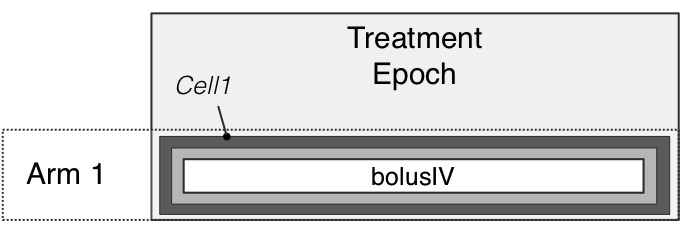
\includegraphics[width=0.7\linewidth]{pics/designPattern_1Arm1Epoch_Ribba}
\caption{Design overview: single arm design.}
\label{fig:1Arm1Epoch_RibbaDesign}
\end{figure}

\begin{figure}[ht!]
\centering
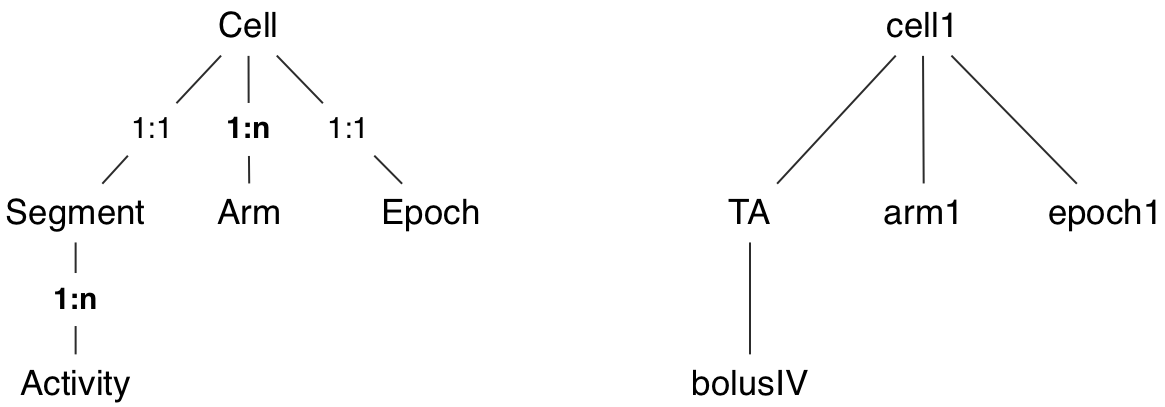
\includegraphics[width=0.7\linewidth]{pics/cellHierarchy_Ribba}
\caption{General cell hierarchy (left); The root of the trial design structure hierarchy is the 'Cell' which can contain one 'Segment',
one 'Epoch' and multiple 'Arms'. The 'Segment' element can have multiple child elements, the 'Activities', e.g. treatments or a washout. (right) An example of how it is applied in \cite{Ribba:2012uq}.}
\label{fig:cellHierarchy_Ribba}
\end{figure}

\begin{table}[htdp!]
\begin{center}
\begin{tabular}{ccccccc}
\hline
Segment&Activity & Treatment & DoseTime & DoseSize & Target Variable \\
\hline
TA& bolusIV &  IV bolus & individual & 1 & C \\
\hline
\end{tabular}
\end{center}
\caption{Segment/activity overview.}
\label{tab:segementActivity_Ribba}
\end{table}

%%%%%%%%%%%%%%%%%%%%%%%%%%%%%%%%%%%%%%%%%%%%%%%%%%%%%%%%%%%%%%%%
\subsubsection{Population}
In the next step, the \textit{Population} is defined, i.e. attributes of the individuals in the study. 
This means creating an individual template with columns for an identifier, arm and repetition and then
populating the table with appropriate data.
As no covariates are used here the \textit{Population} description reduces to the assignment 
of the subjects to the single study arm, \textit{Arm1}. As a shorthand we use the
\textit{repetition} method by defining the column 'rep', as can be seen in the following listing 
\inputxml{Ribba_population.xml}
The identifiers, ID, created here are unique and will be used to the refer to specific subjects 
in the subsequent \xelem{IndividualDosing} structure element described in the following section.


%%%%%%%%%%%%%%%%%%%%%%%%%%%%%%%%%%%%%%%%%%%%%%%%%%%%%%%%%%%%%%%%
\subsubsection{Individual Dosing}
\label{subsubsec:Ribba_indivDosing}

This model utilises the idea of the so called K-PK model, meaning that the rate of the drug entry is relevant
but not its absolute value. Such models often assume, as it is the case here, that the dose is equal 1
for all subject and dosing events, see Table \ref{tab:Ribba_dataSet}.

\begin{table}[htdp]
\begin{center}
\begin{tabular}{rrrr | rrrr | rrrr}\toprule
ID&TIME&DV&DOSE & ID&TIME&DV&DOSE& 			ID&TIME&DV&DOSE \\\midrule
1&0&.&.& 		 	1&116.23&72.04&.& 				20&13.4&.&1\\
1&3.43&45.7&.& 	1&121.87&90.16&.& 				20&17.13&42.62&.\\
1&5.3&48.03&.& 	$\dots$ &$\dots$ &$\dots$ & $\dots$&	21&0&.&.\\
1&42.13&71.34&.& 	$\dots$ &$\dots$ &$\dots$ & $\dots$&	21&1.5&.&1\\
1&52.63&79.3&.& 	20&0&48.61&.&					21&3.17&.&1\\
1&54.57&.&1 & 	20&4&.&1&						21&4.85&.&1\\
1&57.53&72.3&.& 	20&5.88&.&1&						21&6.52&.&1\\
1&59.77&.&1 & 	20&6.7&46.64&.&					21&8.19&.&1\\
1&63.3&72.07&.& 	20&7.76&.&1&						21&9.77&72.35&.\\
1&68.97&70.24&.& 	20&9.27&44.97&.&					21&9.87&.&1\\
1&76.53&66.81&.& 	20&9.64&.&1&						21&14.23&66.96&.\\
1&94.53&60.48&.&	20&11.52&.&1&					21&18.13&56.79&.\\
1&106.1&62&.& 	20&13.23&42.96&.&					21&23.9&60.06&.\\\bottomrule
\end{tabular}
\end{center}
\caption{Data used in \cite{Ribba:2012uq}, an excerpt from the experimental data set in NONMEM format. 
The columns are: the identifier, ID, time for measurements and dosing events, 
dependent variable, DV, which stand for \var{PSTAR} -- the total tumour size and 
the dose, DOSE. As common for K-PD models, the dose is equal 1 for all subjects and 
dosing events.}
\label{tab:Ribba_dataSet}
\end{table}%

The element \textit{IndividualDosing} is used to implementing all such subject specific
dosing events. First we have to associate the data which follow to an appropriate activity,
this is done by referring to the 'bolusIV' which defined previously in \xelem{Structure}, as 
as shown in the following listing \inputxml{Ribba_individualDosing.xml}
Next we map the subject's identifier \var{ID} to that created in the population definition. 
Finally a data set template using \xelem{Definition} element is defined, 
i.e. the columns \var{ID}, \var{TIME} and \var{DOSE}.
Then the table is populated with subject specific values as shown here for subjects 1, 2 and 21.


%%%%%%%%%%%%%%%%%%%%%%%%%%%%%%%%%%%%%%%%%%%%%%%%%%%%%%%%%%%%%%%%
\subsection{Structural model definition}
The following ODE system is defined:
\begin{align*}
\frac{dC}{dt} &= -\textit{KDE} \times C  \nonumber \\
\frac{dP}{dt} &= \lambda_P \times P \Big( 1 - \frac{P^\star}{K} \Big) + k_{\textit{QPP}} \times Q_P - k_{\textit{PQ}} \times P - \gamma \times C \times \textit{KDE} \times P  \nonumber \\
\frac{dQ}{dt} &= k_{PQ}\times P - \gamma \times C\times \mathit{KDE}\times Q \nonumber \\
\frac{dQ_P}{dt} &= \gamma \times C \times \textit{KDE} \times Q - k_{\textit{QPP}} \times Q_P - \delta_{\textit{QP}} \times Q_P  \nonumber \\ \nonumber \\
P^{\star} &= P + Q + Q_P \nonumber
\end{align*}
with initial conditions
\begin{align*}
C(t=0) = 1; \quad P(t=0) = P0; \quad Q(t=0) = Q0; \quad Q_P(t=0) = 0.  \nonumber
\end{align*}

%%%%%%%%%%%%%%%%%%%%%%%%%%%%%%%%%%%%%%%%%%%%%%%%%%%%%%%%%%%%%%%%
\subsubsection{Defining initial conditions}
This example differs from the previous ones. It requires, in addition to model parameters, 
the estimation of the initial conditions of two tumour growth related variables. 
Moreover, the inter-individual variability is assumed for these variables.
The value for $Q_P(t=0)=Q_{P_0}$ is fixed to $0$ but the values for $P(t=0)=P_0$ and $Q(t=0)=Q_0$
are allowed to vary according to a log-normal distribution, see the following listing 
\inputxml{Ribba_initialConditionsDef.xml} where the definition of the distribution for the 
initial condition $P_0$ is shown.



%%%%%%%%%%%%%%%%%%%%%%%%%%%%%%%%%%%%%%%%%%%%%%%%%%%%%%%%%%%%%%%%
\subsection{Modelling steps}
This requires the specification of the following items: \textit{EstimationStep} and \textit{StepDependencies}.
It has been described in previous examples in detail and will be skipped here.


%%%%%%%%%%%%%%%%%%%%%%%%%%%%%%%%%%%%%%%%%%%%%%%%%%%%%%%%%%%%%
%\begin{table}[htdp!]
%\begin{center}
%\begin{tabular}{cc}
%\hline
%Arm & N \\
%\hline
%Arm 1 & 21\\
%\hline
%\end{tabular}
%\end{center}
%\label{default}
%\caption{Arm definition}
%\end{table}%

%
%
%\begin{table}[htdp!]
%\begin{center}
%\begin{tabular}{p{0.3\textwidth}}
%%\hline
%\hline
%\small
%Cell 1
%\begin{itemize} \itemsep1pt \parskip0pt \parsep0pt
%\item
%Arm 1
%\item
%Epoch1
%\item
%Segment TA
%\begin{itemize} \itemsep1pt \parskip0pt \parsep0pt
%\item
%Activity -- IV
%\end{itemize}
%\end{itemize} \\
%\hline
%\end{tabular}
%\end{center}
%\label{default}
%\caption{Cell/Segment/Activity/Arm/Epoch overview}
%\end{table}%


%
%%%%%%%%%%%%%%%%%%%%%%%%%%%%%%%%%%%%%%%%%%%%%%%%%%%%%%%%%%%%%
%\begin{table}[htdp]
%\begin{center}
%\begin{tabular}{lcccc}
%\hline
%Treatment &  Administration Type & DoseTime & DoseSize & Target Variable \\
%\hline
%Treatment A &  OR bolus & \text{individual} & \text{individual} & C \\
%\hline
%\end{tabular}
%\end{center}
%\label{default}
%\caption{Dosing overview}
%\end{table}%
%
%%%%%%%%%%%%%%%%%%%%%%%%%%%%%%%%%%%%%%%%%%%%%%%%%%%%%%%%%%%%%
%\begin{table}[htdp]
%\begin{center}
%\begin{tabular}{cc}
%\hline
%Arm & N \\
%\hline
%Arm 1 & 21\\
%\hline
%\end{tabular}
%\end{center}
%\label{default}
%\caption{Arm definition}
%\end{table}%


%
%\eglabel{10}
%\section{Example \theexamples: Higher levels of variability}
%
%When using the data-set to define the trial design then it is possible
%to in this way to define many more levels of variability than are
%shown here. To do this you simply need to define the variability
%lebels you need using the \xelem{VariabilityLevel} elements at the
%start of the model definition and then map your data-set to each of
%these variability levels using the \xelem{UseVariablityLevel} element
%in the mapping parts of the Estimation or Simulation step.

%%% Local Variables:
%%% mode: latex
%%% TeX-master: "../moml-specification"
%%% End:


%%%%%%%%%%%%%%%%%%%%%%%%%%%%%%%%%%%%%%%%%%%%%%%%%%%%%%%%%%%%%%%%%
%\subsection{Modelling Steps}
%
%By now you must be familiar with how we map data in a data-set
%\index{data-set} to the
%rest of the model. This model follows the approach that you have
%seen, but we have not had a model with multiple levels of
%variability or categorical covariates before so how \pharmml handles
%these features needs some explanation.
%
%\begin{table}[htb]
%\centering
%\begin{tabular}{r r r r r r r r}\toprule
%id&Ttme&Y&dose&occ&treat&sex&streat\\\midrule
%1 &	0 &	. &	4 &	1 &	A &	M &	A-B\\
%1 &	0.25 &	2.1243964 &	. &	1 &	A &	M &	A-B\\
%1 &	0.5 &	4.308573 &	. &	1 &	A &	M &	A-B\\
%1 &	1 &	7.6059305 &	. &	1 &	A &	M &	A-B\\
%1 &	2 &	6.9678311 &	. &	1 &	A &	M &	A-B\\
%1 &	0 &	. &	4 &	2 &	B &	M &	A-B \\
%1 &	0.25 &	4.2049182 &	. &	2 &	B &	M &	A-B\\
%1 &	0.5 &	7.2508737 &	. &	2 &	B &	M &	A-B\\
%1 &	1 &	8.5792413 &	. &	2 &	B &	M &	A-B\\
%1 &	2 &	8.5689542 &	. &	2 &	B &	M &	A-B\\
%31 &	0 &	. &	4 &	1 &	B &	F &	B-A\\
%31 &	0.25 &	3.7113248 &	. &	1 &	B &	F &	B-A\\
%31 &	0.5 &	5.0077184 &	. &	1 &	B &	F &	B-A\\
%31 &	1 &	8.9052428 &	. &	1 &	B &	F &	B-A\\
%31 &	2 &	6.8447695 &	. &	1 &	B &	F &	B-A\\\bottomrule
%\end{tabular}
%\caption{An excerpt of the data-file used to define the IOV estimation.}
%\label{tab:eg6-estdata}
%\end{table}
%
%The data-set we need to map to the model is shown in table
%\ref{tab:eg6-estdata}. Our first task is to inform \pharmml that the
%\dscol{id} and \dscol{occ} columns define the variability of the
%model. We do this using the \xelem{UseVariabilityLevel} we first saw
%in example \egref{3} (section \ref{sec:eg3-simdata-mapping}). Listing
%\ref{eg:eg6-ms-prt1} shows how we use this column twice, first to map
%the \dscol{id} column to the \attval{indiv} variability level and
%second to map the \dscol{occ} column to the \attval{occ1} variability
%level. Each unique value in the respective column is taken to indicate
%a variability node within each level of variability (see section
%\ref{sec:variabilityModel}).
%
%\begin{listing}[htb]
%\inputxml{eg6_ms_prt1.xml}
%\caption{The data-set and variability mapping in example \egref{6}.}
%\label{eg:eg6-ms-prt1}
%\end{listing}
%
%In listing \ref{eg:eg6-ms-prt1} we also see how the categorical
%covariate \var{Treat} is populated by the \dscol{treat} column of the
%dataset. Note for this to work the values in the column must
%correspond \emph{identically} to the names of the covariate's
%categories. In this case the covariate \var{Treat} has category
%\var{A} and \var{B} so this works.
%
%\begin{listing}[htb]
%\inputxml{eg6_ms_prt2.xml}
%\caption{The complex covariate mappings in example \egref{6}.}
%\label{eg:eg6-ms-prt2}
%\end{listing}
%
%Listing \ref{eg:eg6-ms-prt2} shows us how we deal with cases where the
%content of the data-set does not match the category name. In this
%cases the covariate is \var{TreatSeq}, which has two categories:
%\var{AB} and \var{BA}. In the data-set these are encoded as
%``\texttt{A-B}'' and ``\texttt{B-A}'' respectively. By now hopefully
%you know what to expect. We use a conditional expression to identify
%the values we are interested in. In this first mapping this is the
%string ``\texttt{A-B}''. What is new in this mapping is the
%\xelem{Assign} element. We use this to assign the string value
%``texttt{AB}'' to the covariate, which matches the \var{AB}
%category. We take the same approach to map the other category of
%\var{TreatSeq} and the categories of the \var{Occ} covariate, although
%the latter is not shown here.
%
%
%\eglabel{7}
%\section{Example \theexamples: Estimation with IOV, explicitly defined trial design}
%\label{eg7:example7}
%
%%%%%%%%%%%%%%%%%%%%%%%%%%%%%%%%%%%%%%%%%%%%%%%%%%%%%%%%%%%%%%%%%
%\subsection{Description}
%
%This example is identical to example \egref{6} except that the trial
%design is defined explicitly within the \xelem{Design} element of the
%\pharmml document. This trial design also introduces some concepts
%that we have not seen in previous examples.
%
%%%%%%%%%%%%%%%%%%%%%%%%%%%%%%%%%%%%%%%%%%%%%%%%%%%%%%%%%%%%%%%%%
%\subsection{Trial Design}
%
%The trial design being represented here is described in detail in
%example \egref{6} (see also figure \ref{fig:eg6-crossover-design} and
%section \ref{sec:eg6}). We have omitted the
%\xelem{Treatment} elements in listing \ref{eg:eg7-td-prt1} because we
%want to focus on the parts we have not discussed before. Here the
%\xelem{TreatmentEpoch} \attval{AEp} references treatment A, as in
%previous examples, but it also associates an occasion with the epoch
%sing the \xelem{Occasion} element. Note that the occasion is given an
%identifier, \var{occ1}, and is assigned to a variability level, in
%this case \attval{iov1}. We then use this epoch and the epoch
%\attval{BEp} to define the cross-over study.
%
%\begin{listing}[htb]
%\inputxml{eg7_td_prt1.xml}
%\caption{The trial design of example \egref{7}.}
%\label{eg:eg7-td-prt1}
%\end{listing}
%
%Just Group \attval{a1} is shown in the listing and this defines the
%group as being a sequence of epoch \attval{AEp}, then a washout,
%followed by epoch \attval{BEp}. The ordering in the \xelem{Group}
%element defines the sequence of events. Finally we give an identifier,
%\var{i} for the individuals in this group and assign the individuals
%to a variability level in the model definition. Note that the
%variability level used for \xelem{Individual} must be one level of
%variability higher than that used by the \xelem{Occasion}
%element. At present this section of \pharmml can only describe trials designs
%with at most IOV and IIV.
%
%%%%%%%%%%%%%%%%%%%%%%%%%%%%%%%%%%%%%%%%%%%%%%%%%%%%%%%%%%%%%%%%%
%\subsection{Modelling Steps}
%
%As in examples \egref{1} and \egref{5} we now need to map the data-set
%to the trial design. In particular we need to identify the rows in the
%data-set that define the groups (\attval{a1} and \attval{a2}) and the
%occasions (\attval{occ1} and \attval{occ2}). Listing \ref{eg:eg7-ms}
%shows how we achieve. Using the \xelem{UseVariabilityNode} element we
%tell \pharmml which individual or occasion to use as we read the
%data-set. Since, the structure of the study is defined explicitly,
%this enables \pharmml that the trial design implicitly defined within
%the data-set is consistent with it.
%
%\begin{listing}[htb]
%\inputxml{eg7_ms.xml}
%\caption{Mapping to the trial design in example \egref{7}.}
%\label{eg:eg7-ms}
%\end{listing}
%
%\eglabel{8}
%\section{Example \theexamples: Simulation with IOV, explicitly defined trial design}
%\label{eg8:example8}
%
%%%%%%%%%%%%%%%%%%%%%%%%%%%%%%%%%%%%%%%%%%%%%%%%%%%%%%%%%%%%%%%%%
%\subsection{Description}
%
%This example is in many aspects identical to the previous one, e.g.\ the same structural model and covariates,
%but few features of the trial design and modelling steps are new.
%
%%%%%%%%%%%%%%%%%%%%%%%%%%%%%%%%%%%%%%%%%%%%%%%%%%%%%%%%%%%%%%%%%
%\subsection{Trial Design}
%Here, we define explicitly the start and end times for each epoch and each occasion, see listing \ref{eg:eg8_EpochOccasion_startEnd}.
%In this case the time intervals are identical but this is rather an exception then a rule. Usually, one would have
%multiple occasions within one epoch or the occasion would span over multiple epochs.
%
%\begin{listing}[htb]
%\inputxml{eg8_EpochOccasion_startEnd.xml}
%\caption{Defining start and end times for an epoch and occasion in example \egref{8}.}
%\label{eg:eg8_EpochOccasion_startEnd}
%\end{listing}
%
%Next listing, \ref{eg:eg8_groupSize} shows how to describe a group, here with three epochs, treatments and one washout in between,
%and the number of subjects in this group.
%As explained in the Trial Design chapter, section \ref{sec:CTS}, the 'Washout' epoch means complete reset of all
%drug amounts and is defined without start and end times.
%
%\begin{listing}[htb]
%\inputxml{eg8_groupSize.xml}
%\caption{Defining group, i.e.\ treatment sequence and number of subjects in example \egref{8}.}
%\label{eg:eg8_groupSize}
%\end{listing}
%
%%%%%%%%%%%%%%%%%%%%%%%%%%%%%%%%%%%%%%%%%%%%%%%%%%%%%%%%%%%%%%%%%
%\subsection{Modelling steps}
%The number of observations time points at which the observation variable is to be estimated, here \textit{Cc}, is defined
%using a construct seen before in listing \ref{eg:eg5-trial-design-vals} in the definition of the dosing time sequence.
%Here the time sequence is uniqely specified by providing the
%\begin{itemize}
%\item
%start time, \textit{begin}
%\item
%number of equidistant intervals, \textit{repetitions}
%\item
%length of each interval, \textit{stepSize}
%\end{itemize}
%
%
%\begin{listing}[htb]
%\inputxml{eg8_modellingSteps.xml}
%\caption{Defining \textit{Observations} and \textit{StepDependencies} in example \egref{8}.}
%\label{eg:eg8_modellingSteps}
%\end{listing}
%
%
%\eglabel{9}
%\section{Example \theexamples: Simulation with IOV, trial design specified in a data file}
%
%This example is identical as the previous one except that the trial design is specified by the experimental data file.
%The major consequences are that
%\begin{itemize}
%\item
%the \xelem{Design} block is missing
%\item
%we have to define the external data source, see listing \ref{eg:eg9_dataSet}
%\item
%and instead of defining the \xelem{Observations} we have the \xelem{SimDataSet} block to interpret the data-set,
%listing \ref{eg:eg9_simDataSet}, described in detail in section \ref{sec:eg3-simdata-mapping}.
%\end{itemize}
%
%
%\begin{listing}[htb]
%\inputxml{eg9_dataSet.xml}
%\caption{Defining external data source in example \egref{9}.}
%\label{eg:eg9_dataSet}
%\end{listing}
%
%
%\begin{listing}[htb]
%\inputxml{eg9_simDataSet.xml}
%\caption{Defining \xelem{SimDataSet} block to interpret the data-set in example \egref{9}.}
%\label{eg:eg9_simDataSet}
%\end{listing}
%
%\clearpage
%%\newpage


%%% Local Variables:
%%% mode: latex
%%% TeX-master: "../moml-specification"
%%% End:



